
\chapter{MonteCarlo simulation tools}

As a second approach to the characterization of scintillating crystals in the aspects that influence timing, Monte Carlo simulation tools have been taken into account. Indeed, the domain of application of ray tracing software is somewhat limited, as will be clear after the discussion in this chapter. Nonetheless it retains a certain importance for what concerns the understanding of the components of resolution loss when it comes to optical propagation of photons. Two software packages have been considered and reviewed \cite{Pizzi2012}: Geant4 and SLitrani.

\section{Ray tracing}

The software available and reviewed, that is Geant4 and SLitrani, broadly share the same approach in terms of ray tracing in optical materials. 
The photon is treated as a particle travelling inside the volume and interacting via precise processes, such as absorption in the bulk, scattering, wavelength shifting and boundary interaction. 
Effective models are applied when it comes to optical photon production and no theoretical implementation of fluorescence phenomena is implemented. In particular we can articulate the approach to ray tracing in three steps:
\begin{itemize}
\item the energy deposition model, that defines the voxelized map of the energy deposited with a certain cut value for processes
\item the production phase, where the energy deposition map is translated into a number of optical photons at a certain predefined wavelength, with a resolution spread
\item the ray tracing phase, where the produced photons are tracked to the end of the volume or until absorption takes place
\end{itemize}
Before defining the different approaches of the two software packages it is necessary to briefly discuss some theoretical aspects of optical photon interaction in possible tracking volumes: Rayleigh scattering and interaction at boundaries.

\subsection{Rayleigh scattering}

The Rayleigh scattering is the elastic scattering of light or other electromagnetic radiation by particles much smaller than the wavelength in exam.
It can be described in a classical way as a result of electric polarizability of particles.
The particle indeed behaves as a small radiating dipole as the electric field of the light wave acts on the charge. We just here quote the Rayleigh cross section, which is 
\begin{equation}
\sigma _{Rayleigh} = \frac{2\pi ^{2}}{3} \frac{d^{6}}{\lambda ^{4}}\left( \frac{n^{2}-1}{n^{2}+2} \right) ^{2}
\end{equation}
where $\lambda$ is the wavelength, d is the characteristic size of the scattering center and n is the refractive index of the medium.
It is not evident to identify scattering processes inside heavy scintillator crystals as Rayleigh interactions and this is beyond the scope of this work. Nevertheless the toolkits analysed and used in this study specify a scattering length of Rayleigh processes, and this is necessary to account for scattering inside the bulk, which, as will be seen by measurement performed, is of foremost importance.

\subsection{Model for surface interactions}
Surface interaction proved to be quite hard to model. As a photon hits a boundary, it can be absorbed, transmitted or reflected depending on the  materials at both sides of the boundary. This involves optical properties, such as the index of refraction and the absorption coefficient as well as surface properties of the material, such as roughness or shape.
Modelling these parameters, and obtaining them via measurements is quite difficult, and ray tracing software often implement effective models, with limited applicability.
In addition, crystals may present anisotropic properties, thus requiring the implementation of wave models rather than simple particle tracking.
In this study we will not consider such a property, and in the case of small pixels it can usually be neglected \cite{Cuccia2013}.

A simple solution is the definition of border surfaces as ordered pairs of physical volumes. In case of simple polished surfaces between two dielectric materials, the only relevant property is the index of refraction.
In case the surface is painted or wrapped the definition may include the index of refraction of the thin layer. This allows for Lambertian (diffused) or specular refraction to take place at the back of the layer. By defining combination of surface finish properties it is possible to grossly model the experimental conditions.

A more refined though incomplete solution implements the so called \textit{Unified} model.  
It is usually defined for dielectric-dielectric interfaces and it considers the surface to be made up of micro-facets with normal vectors that follow given distributions around the nominal normal for the volume at the impact point.

This models are implemented in SLitrani and Geant4, but given the limited applicability due to lack of data about surfaces, only more simple approaches have been evaluated, modelling reflection at boundaries as Lambertian or specular at the expenses of accuracy.

\section{Geant4}
Geant4 is a toolkit for simulating the passage of particles through matter, based on C++ language. It includes a comprehensive range of features, including electromagnetic, hadronic and optical processes, a large set of long-lived particles, materials and elements from hundreds of eV to the TeV scale.
An analysis of Geant4 extended capabilities is beyond the scope of this work, a review can be find in \cite{Agostinelli2003}.
For what concerns optical photons production and ray tracing a brief introduction is given below.

\subsection{Physics}
An optical photon is characterized by a wavelength much greater than the typical atomic spacing.
In Geant4 optical photons are treated as a separate class, so to include wave-like properties into the processes.
Since the description breaks down at higher energies, there is no smooth transition as a function of energy between the optical photon and $\gamma$ particle classes.
Ray tracing in Geant4 has the following characteristics:
\begin{itemize}
\item \textbf{Energy deposition scheme}: it implements complex models for the different particles and provides for tracking of secondaries. Many different pre-defined packages are included to describe processes at different energy scales, including low energy electromagnetic phenomena. 
In this work the G4Livermore libraries have been used, which are optimised for precise treatment of EM showers and interactions at low energy (keV scale). They guarantee the best accuracy until 250 eV, at the cost of a more CPU-intensive simulation. Processes implemented include polarized Compton scattering, polarized photo electric effect, ionization and bremsstrahlung for electrons. A complete review can be accessed at \cite{Sempau2002}.
\item \textbf{Photon production stage}: optical photons may be produced via a scintillation process or a Cerenkov process. 
A scintillation process may be called after energy deposition in the volume. Indeed, as a secondary goes below threshold for tracking, its energy is deposited in the bulk. Given the optical parameters specified for the material (light yield, resolution scale, time profile of the scintillation, fluorescence spectrum) photons are produced isotropically with random polarization and begin to be tracked with the optical classes.
The Cerenkov process, on the other hand, is called during the simulation step of the tracking of a charged particle over threshold. Frequency and number of photons produced are sampled from the Frank-Tamm formula.
\end{itemize}
When the optical photon is produced, accordingly to the scintillation properties specified for the material, it needs to be tracked to the end of the volume or until it is under threshold for a cut. Polarisation effect can be considered. An optical photon is canonically tracked and can undergo four distinct processes:
\begin{itemize}
\item \textbf{Absorption}: absorption length must be specified at different wavelengths for every material where optical tracking is required. It is a simple exponential decrease in transmitted photons.
\item \textbf{Rayleigh scattering}: Rayleigh scattering length can be specified at different wavelengths for every material where optical tracking is required, and implements the formulas presented before.
\item \textbf{Boundary interaction}: different models are implemented to describe boundary interactions. In particular Fresnel equation are always used to determine the transmission of a single photon given its wavelength, its momentum and the refractive indices of the materials at the boundary.
Moreover, the \textit{Unified} model is implemented for boundaries with wrapping/coatings and air/grease gap.
In this case when a photon arrives at a medium boundary its behaviour depends on the nature of the two materials that join at that boundary. Medium boundaries may be formed between two dielectric materials or a dielectric and a metal. Reflection and transmission probabilities are sensitive to the state of linear polarization. In the case of an interface between a dielectric and a metal, the photon can be absorbed by the metal or reflected back into the dielectric.
However in this study only completely diffusive and reflective wrappings will be considered, with air gap.
\item \textbf{Wavelength shifting}: the user must specify the characteristic length for WLS process, the emission process and time profile. It is not usually necessary to include it in PET like systems.
\end{itemize}

\section{SLitrani}
SLitrani stands for Super LIght TRansmission in ANIsotropic media. It is a general purpose Monte-Carlo program, built upon ROOT \cite{ROOT}, simulating light propagation in any type of set-up which may be represented by the shapes provided by the geometry of ROOT. The first motivation was the characterization of the PbWO$_{4}$ crystals of the ECAL detector at the CMS experiment. As more deeply discussed in \cite{Gentit2002}, this crystal presents high anisotropy that needs to be accounted for.

\subsection{Physics}
Similarly to what happens in Geant4, optical photons are treated as a separate class with respect to high energy particles, so to include wave-like properties into the processes.
\begin{itemize}
\item \textbf{Energy deposition scheme}: includes very basic electromagnetic models for low energy $\gamma$, with Compton scattering and photo electric effect. Coherent scattering is not implemented. Scattered electrons are not tracked: all the energy of the scattered electron emits light at the vertex position where the Compton scattering occurred. 
The cross section for Compton scattering is calculated analytically from the atomic properties of the material.
The photoelectric cross-section must be provided by the user.
In the case of beam of particles, energy deposition is sampled from the dE/dx for the specific material.
\item \textbf{Photon production stage}: scintillation occurs when a particle deposits energy in the bulk of a crystal. So this is affected by the mechanisms previously outlined and the specified characteristics of the material (light yield, resolution scale, time profile of the scintillation, fluorescence spectrum).
Cerenkov effect can be switched on only for charged particle beams of high energy. In this case providing index of refraction n and thickness of material fixes all parameters affecting the generation of Cerenkov light, namely emission angle and number of photons emitted. They are produced with respect to the axis of the beam, without tracking of secondary particles.
\end{itemize}
As previously discussed for Geant4, an optical photon after production is tracked. In the case of SLitrani the tracking is canonical except for boundary interaction, where a wave-like approach is implemented, based on Maxwell equations, thus accounting for anisotropy effect. In this work these effects are not taken into account, and only the case of isotropic crystals is considered. However, as shown in \cite{Cuccia2013} the influence on light collection for small pixels is not significant.
\begin{itemize}
\item \textbf{Absorption}: the management of the process is similar to the one of Geant4, given the input values specified by the user
\item \textbf{Rayleigh scattering}: the management of the process is similar to the one of Geant4, given the input values specified by the user
\item \textbf{Boundary interaction}: SLitrani implements boundary interaction models similar to those of Geant4. There are some differences at a level of the reflection/absorption in the UNIFIED approach that will be quantified in the next section.
The main difference intervenes in the case of anisotropic crystal, where the dielectric tensor is considered, thus accounting for reflections on the different optical planes.
\item \textbf{Wavelength shifting}: the management of the process is similar to the one of Geant4, given the input values specified by the user
\end{itemize}

\section{A comparison for timing simulation}
Since this work is more concerned with the timing implications of detection at low energies, this is the domain were the analysis will be focused.
In this case the main difference between the two software packages comes with the possibility of tracking secondary particles.
In SLitrani the energy deposition models are very simple: scintillation occurs as soon as a photo electric or Compton interaction involves the $\gamma$ quantum.
In the case of Geant4 the implementation, as already seen in the previous section, is more complex. An impinging $\gamma$ deposits energy in the lattice and frees an electron which is able to travel and further ionize the medium.
This implicates that the energy deposited by a quantum in a Geant4 simulation will have a higher spatial spread. This is shown in figure \ref{fig:rms}, where the longitudinal and transversal energy deposition of 511 keV $\gamma$ interacting inside a LSO scintillating crystal of 2x2x20 mm$^{3}$ is compared for the two software packages.
Moreover, secondary electrons of non negligible energy in terms of Cerenkov threshold, can be tracked and photons tracks produced can be simulated. 
\begin{figure}[htbp]
\begin{center}
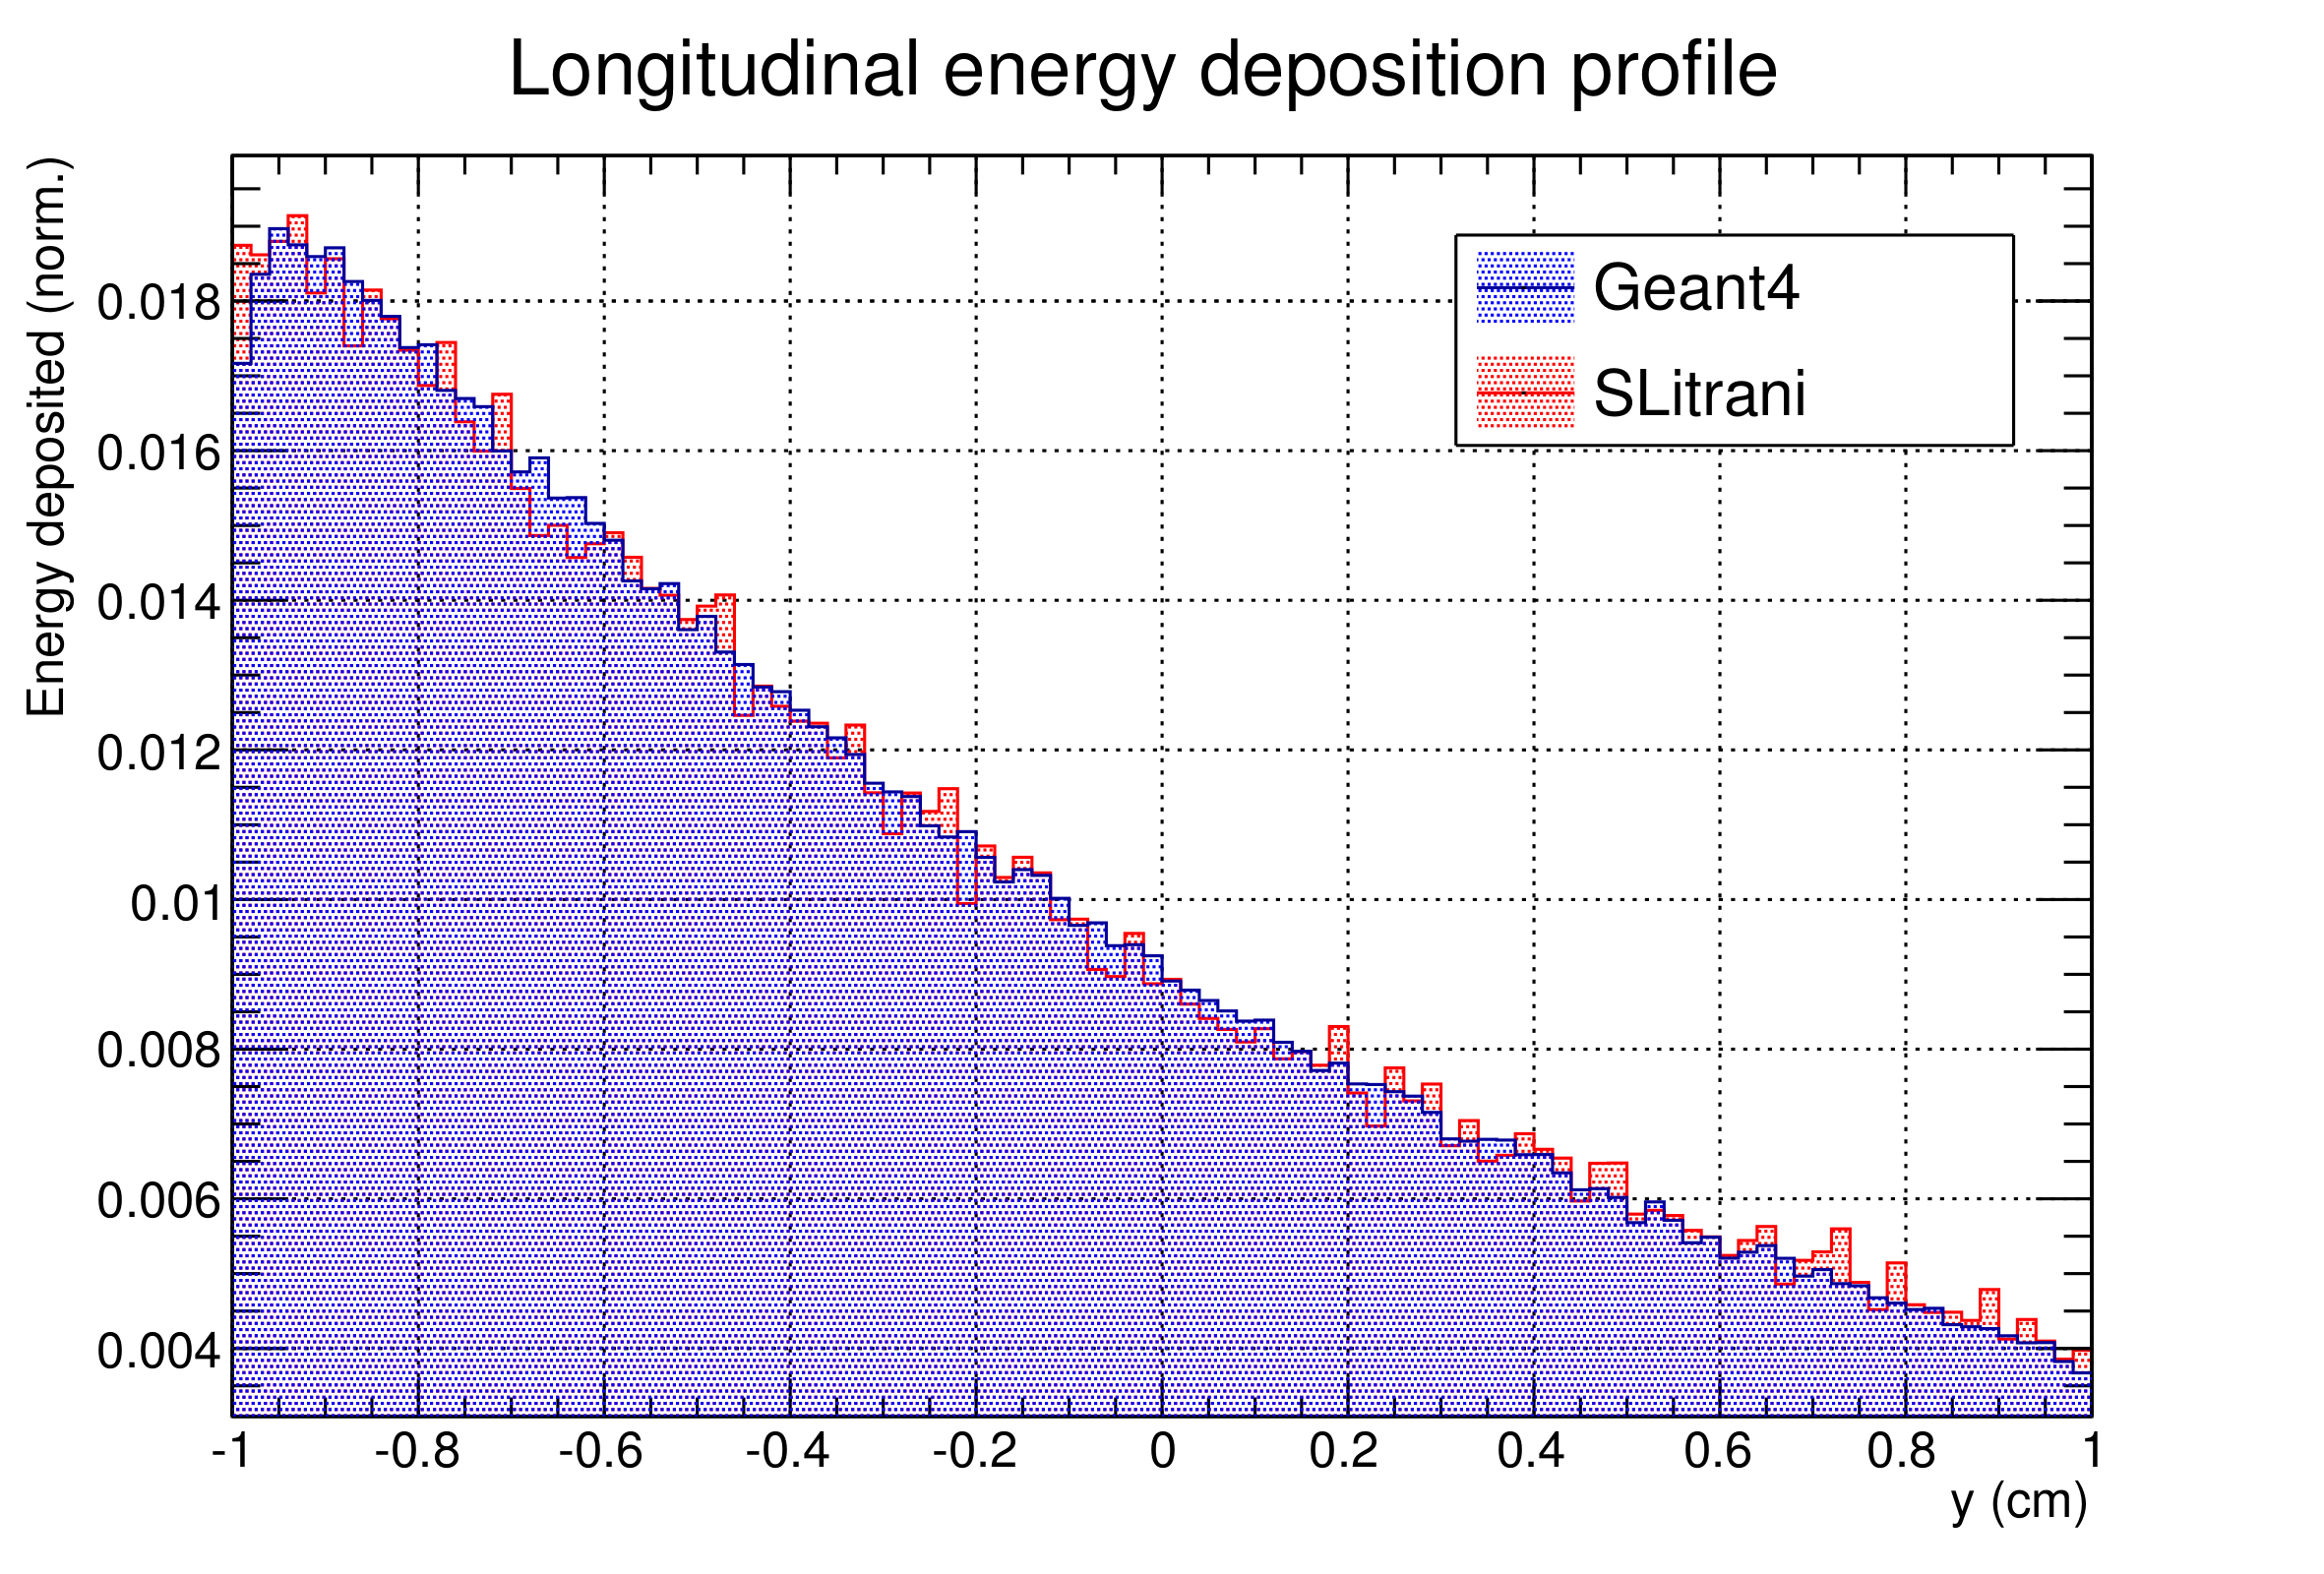
\includegraphics[width=8cm]{../Pictures/Chapter_5/energy_dep.png}
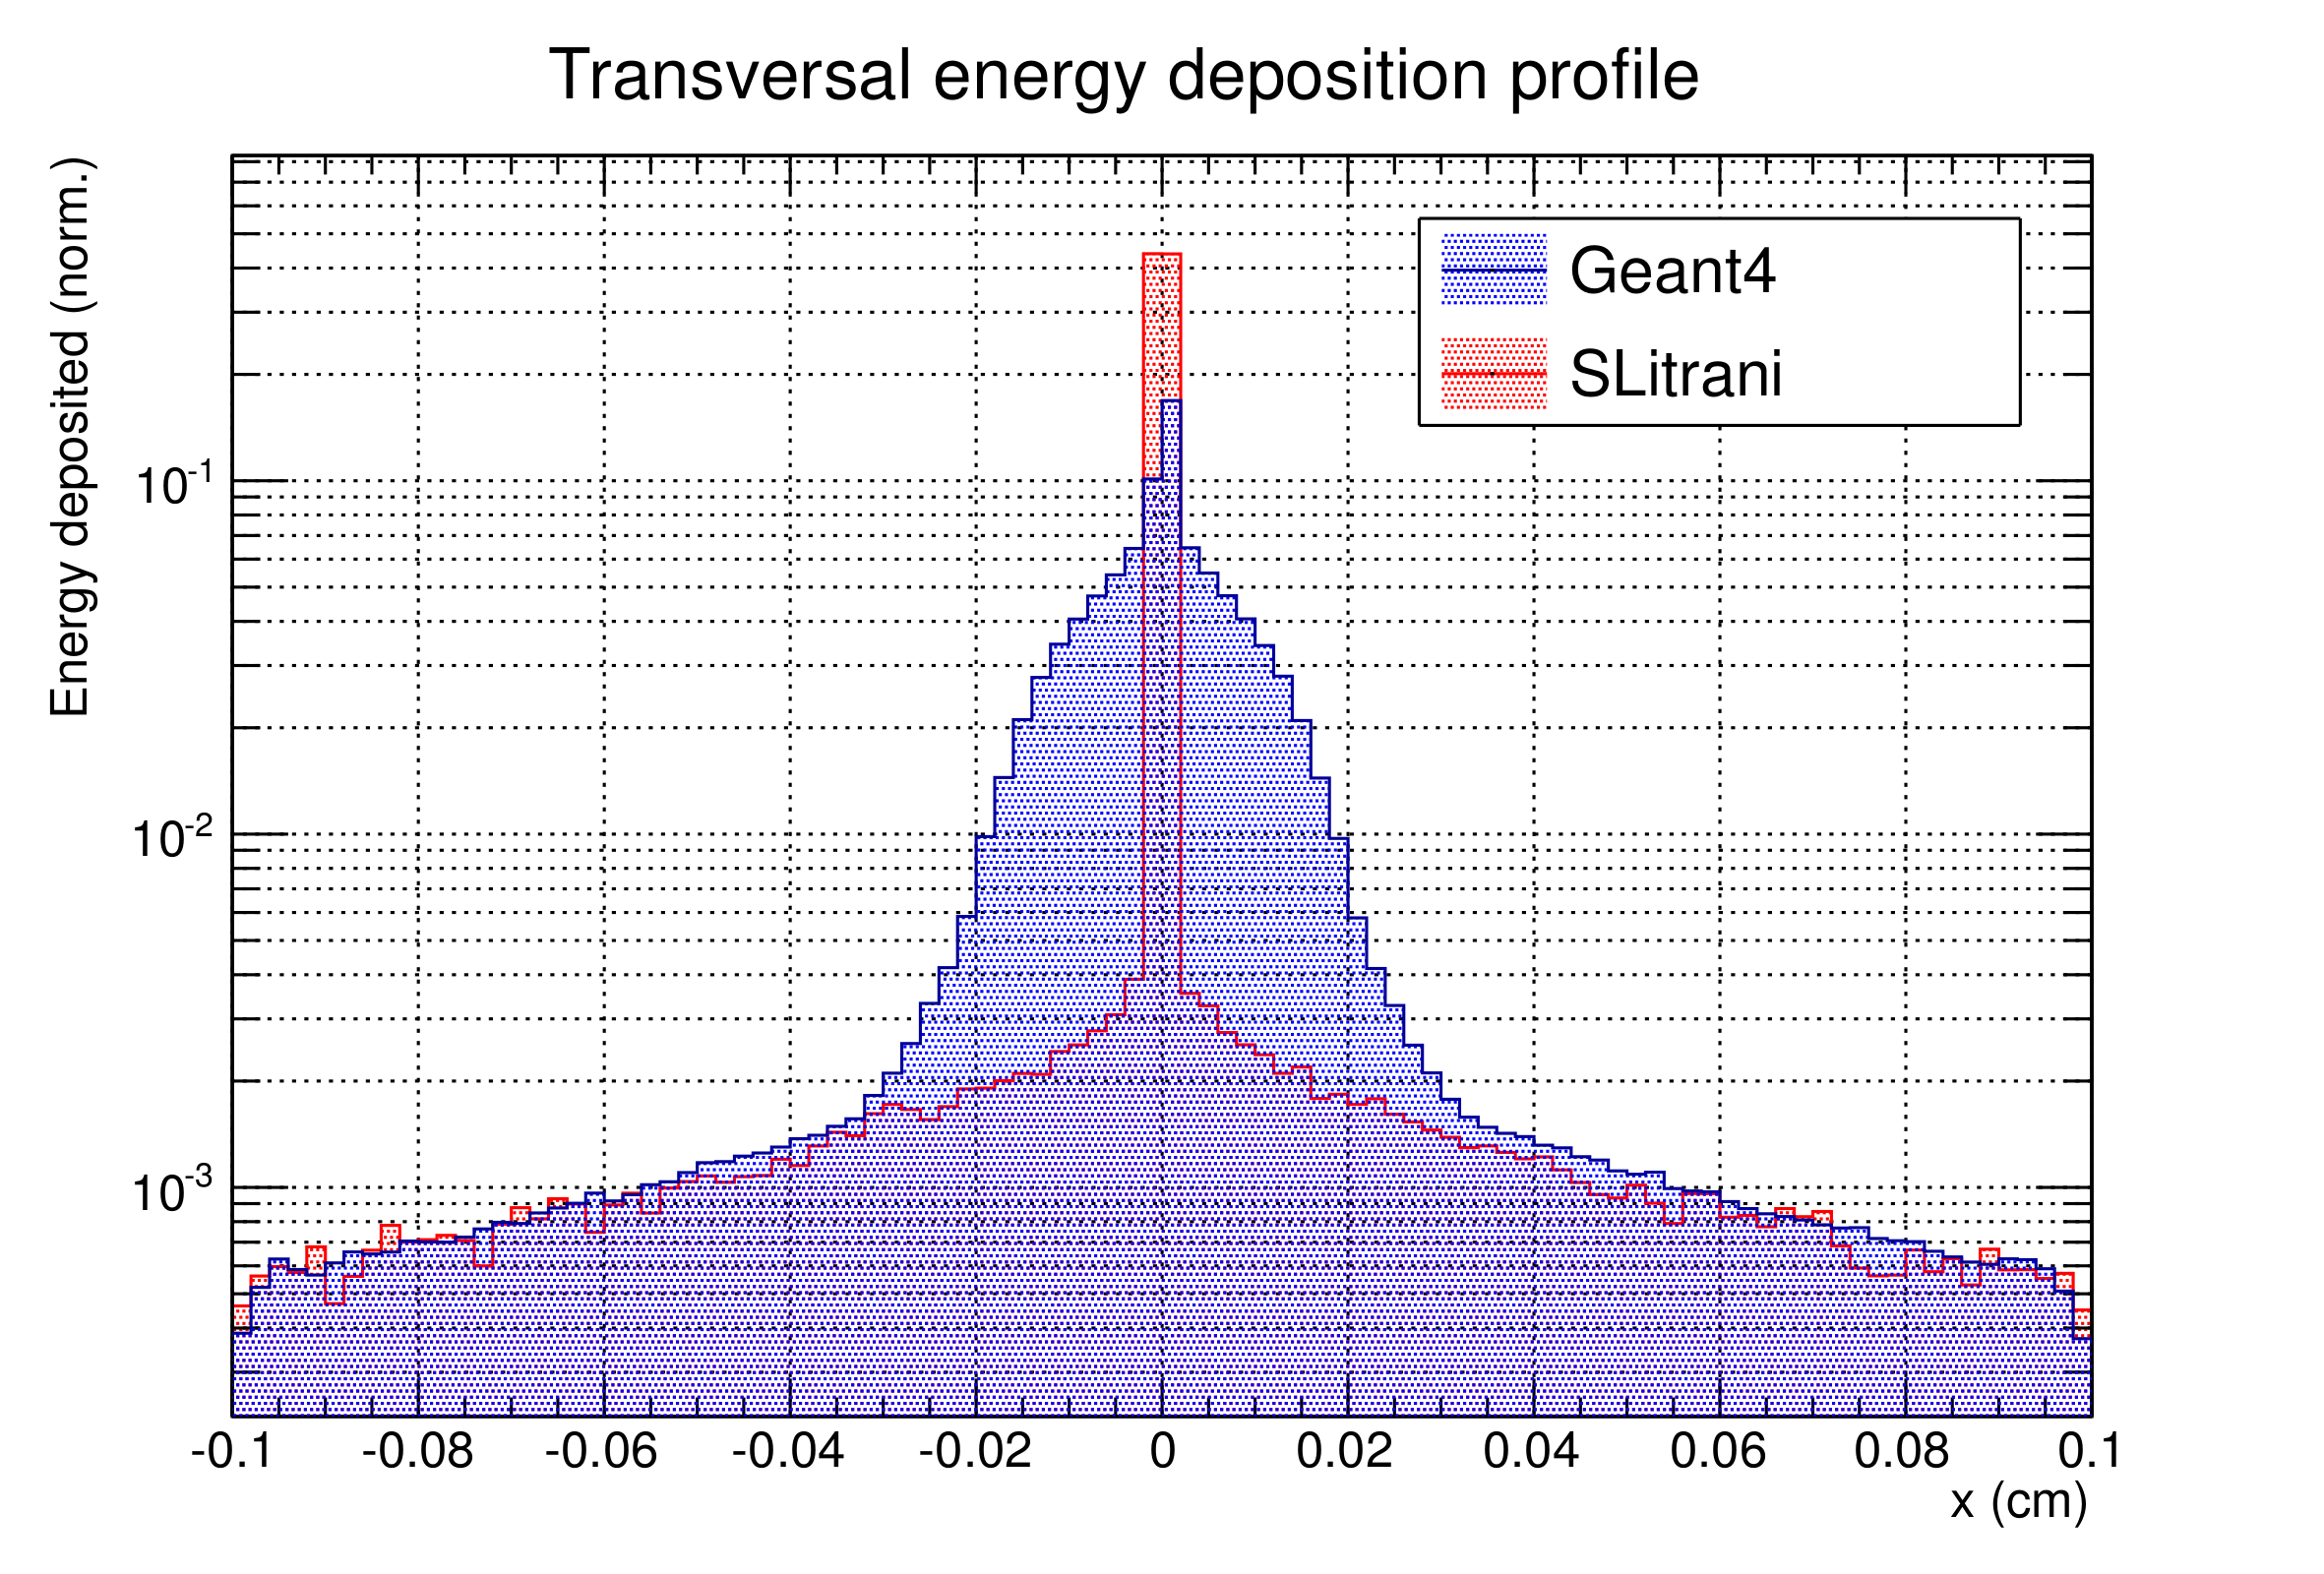
\includegraphics[width=8cm]{../Pictures/Chapter_5/energy_dep_lat.png}
\end{center}
\caption[RMS comparison]{Comparison between energy deposition maps in SLitrani and Geant4 (longitudinal and transversal)}
\label{fig:rms}
\end{figure}
Giving the fact that typical values for light yield of heavy scintillating crystals are around a few tens of thousands photons per MeV, the smearing effect of energy deposition can often be neglected. The same goes for the small amount of Cerenkov photons produced with respect to the number of photons extracted and the subsequent resolution effect.

Nonetheless, as already discussed in the previous chapter, a small but significant impact can be found as soon as timing properties of crystals are taken into account.
\subsection{Cerenkov photons for low energy excitation}
The direction of the Cerenkov photons produced can be neglected, and it retains no value, since the information is completely washed out by the typical path of a low energy electron in the crystalline lattice.
As shown in figure \ref{fig:electron} the path of the electron is tortuous due to the large cross section for multi scattering processes.
\begin{figure}[htbp]
\begin{center}
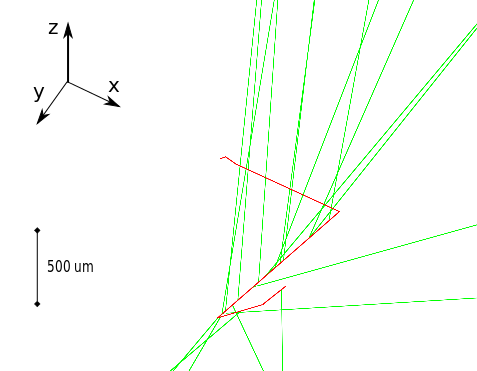
\includegraphics[width=8cm]{../Pictures/Chapter_5/white.png}
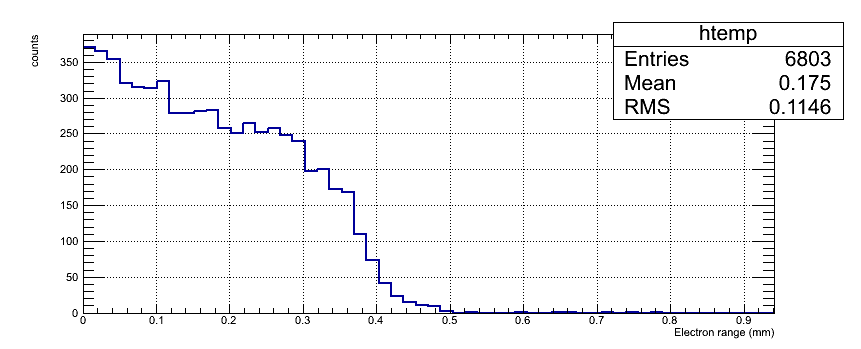
\includegraphics[width=8cm, height=5cm]{../Pictures/Chapter_5/range.png}
\end{center}
\caption[Electron path in lattice]{Example of path of 350 KeV electron in a LSO: Ce lattice (red) and Cerenkov photons produced (green). On the bottom the extracted range of an electron in shown.}
\label{fig:electron}
\end{figure}

On the other hand the first question to be answered when evaluating the impact of Cerenkov photons on time profiles of crystals concerns the number of photons extracted.
It has been shown in chapter 2 that the number of photons produced for different samples may be relevant. 
In order to estimate an order of magnitude for the number of photons collected at the detector, a simulation was performed in Geant4 using the low energy Penelope libraries. The setup is a simple 2x2x3 mm$^{3}$ crystal hit by a 511 KeV $\gamma$ particle. The choice of the sample size was based on the typical experimental conditions in our laboratory. At this stage, the condition were kept as simple as possible, thus including only Fresnel processes and absorption: the crystal is not wrapped and surrounded by air, the coupling medium to the photo detector is air.

\begin{figure}[htbp]
\begin{center}
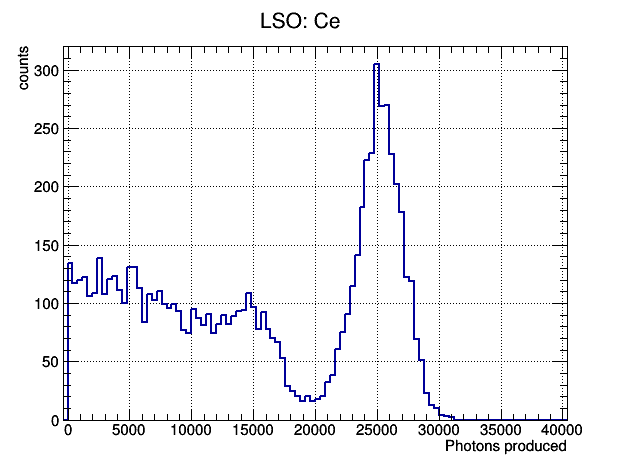
\includegraphics[width=8cm]{../Pictures/Chapter_5/spctrum_LSO.png}
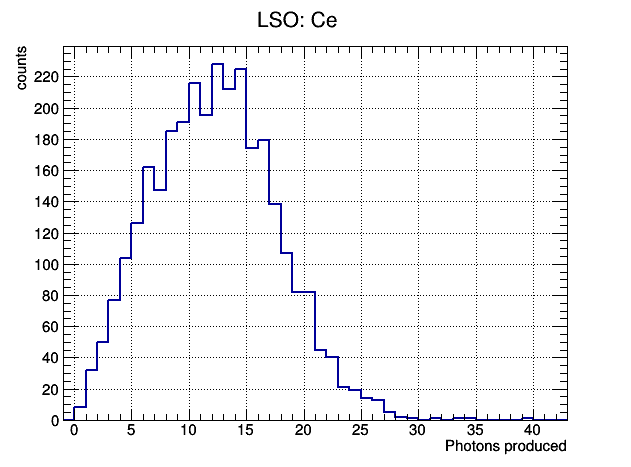
\includegraphics[width=8cm]{../Pictures/Chapter_5/cerenkov_LSO.png}
\end{center}
\caption[LSO photoelectric and Cerenkov production]{Photon production for scintillation processes (left) and Cerenkov production (right)}
\label{fig:ceren_phot}
\end{figure}
As shown in figure \ref{fig:ceren_phot}, the number of Cerenkov photons, which depends essentially on the density and refractive index of the medium is in substantial agreement with the theoretical calculation presented in chapter 2, provided the statistical spread.
Attention should be posed on the fact that this photons are, at the moment, produced, in the range of the scattered electron. 
The number of photons coupled out is substantially reduced by three factors: 
\begin{itemize}
\item the reduced cone of extraction due to the matching of refractive indices (air-crystal)
\item the transmission curve of the crystal
\item the quantum efficiency of the photo detector
\end{itemize}
For what concerns the refractive indices of the materials simulated, values were taken from \cite{Auffray2009}, \cite{Kuwano2004}, \cite{jellison2012}.
The quantum efficiency is wavelength dependent and influences selectively the photons extracted. Therefore it influences the ratio between scintillation and Cerenkov photons detected. Indeed a photo detector more efficient in the UV would collect a higher number of Cerenkov photons. For this preliminary result a standard photo cathode quantum efficiency has been considered, for a Hamamatsu MCP-PMT, between 200 and 1000 nm.
Finally the transmission curve allows only certain wavelengths to be transmitted due to the absorption bands of the crystal. The values extracted have been measured for samples on the crystalline species used with the method outlined in the next sections.
\begin{table}[h]
\begin{center}
\begin{tabular}{|l|l|l|l|}
\hline
Crystal  & Calculated & Produced & Collected \\
\hline
LSO: Ce  & 15         & 12.1     & 1.4       \\
\hline
PbWO4    & 21         & 18       & 4.1       \\
\hline
LuAG: Ce & 25         & 20       & 6         \\
\hline
CeF3     & 13         & 14       & 1           \\
\hline
BGO      & 23         & 25       & 3.2     \\ 
\hline
\end{tabular}
\end{center}
\caption[Cerenkov photons produced in common crystals]{Example of Cerenkov photons calculated and simulated (produced and collected) for different crystals. The values are already corrected for the quantum efficiency over the emission range.}
\label{table:cer}
\end{table}
This small number can be neglected in most cases: the role of these photons becomes less and less relevant as the time constants of the crystal get fast. For main  scintillators, Cerenkov photons produced and collected are shown in table \ref{table:cer}. This is in agreement with previous studies, such as \cite{Brunner2014}.

In particular they are negligible when the ratio between Cerenkov photons collected and scintillation photons collected becomes low. In this case most of the photons collected come from a scintillation event.
When dealing with PET like setups one should also take into account the fact that selection on the photopeak usually is mandatory for improving the signal to noise ratio. This changes also the ratio between Cerenkov and scintillation photons, since it is much more likely for a photoelectric event to couple out a Cerenkov photon produced by the secondaries (as shown in figure \ref{fig:ceren_pp}). This is given by the fact that a photo electric effect extract a single electron from a deep shell over threshold for Cerenkov effect.

\begin{figure}[htbp]
\begin{center}
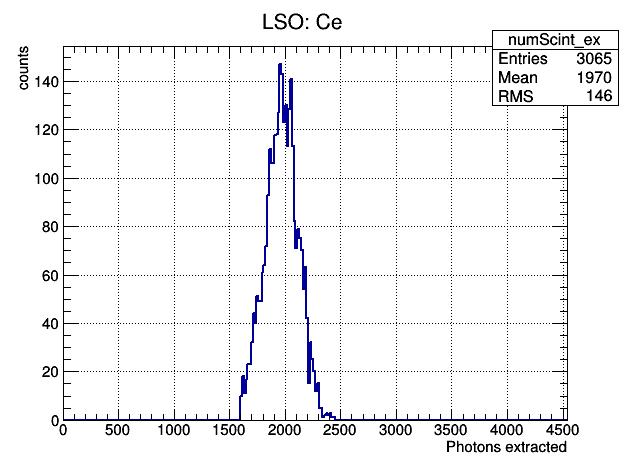
\includegraphics[width=8cm]{../Pictures/Chapter_5/pp_LSO.png}
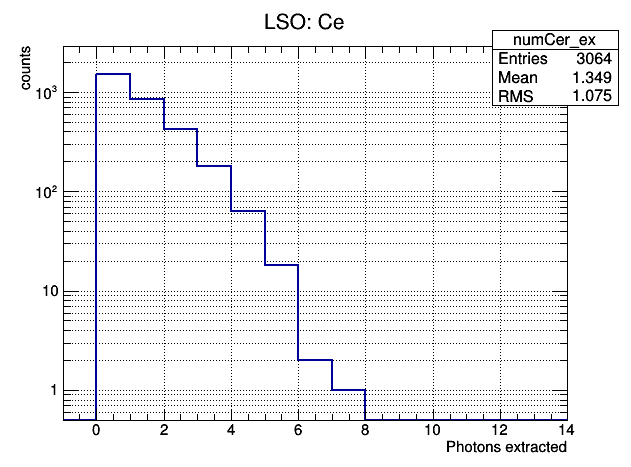
\includegraphics[width=8cm]{../Pictures/Chapter_5/cer_extr_LSO.png}
\end{center}
\caption[Photopeak selection for Cerenkov simulation]{The spectrum is selected on the LSO photo peak (top) and the number of Cerenkov collected changes slightly with respect to figure \ref{fig:ceren_phot} (bottom)}
\label{fig:ceren_pp}
\end{figure}
\newpage
As a final remark it is interesting to underline the timing characteristics of the Cerenkov spectrum. Indeed these photons are produced promptly and they can influence, albeit slightly, the time resolution. They can especially change the way we set thresholds on events.
As shown in figure \ref{fig:time_ratio} in the first 100 ps a relevant part of the photons collected is taken by Cerenkov photons.
\begin{figure}[htbp]
\begin{center}
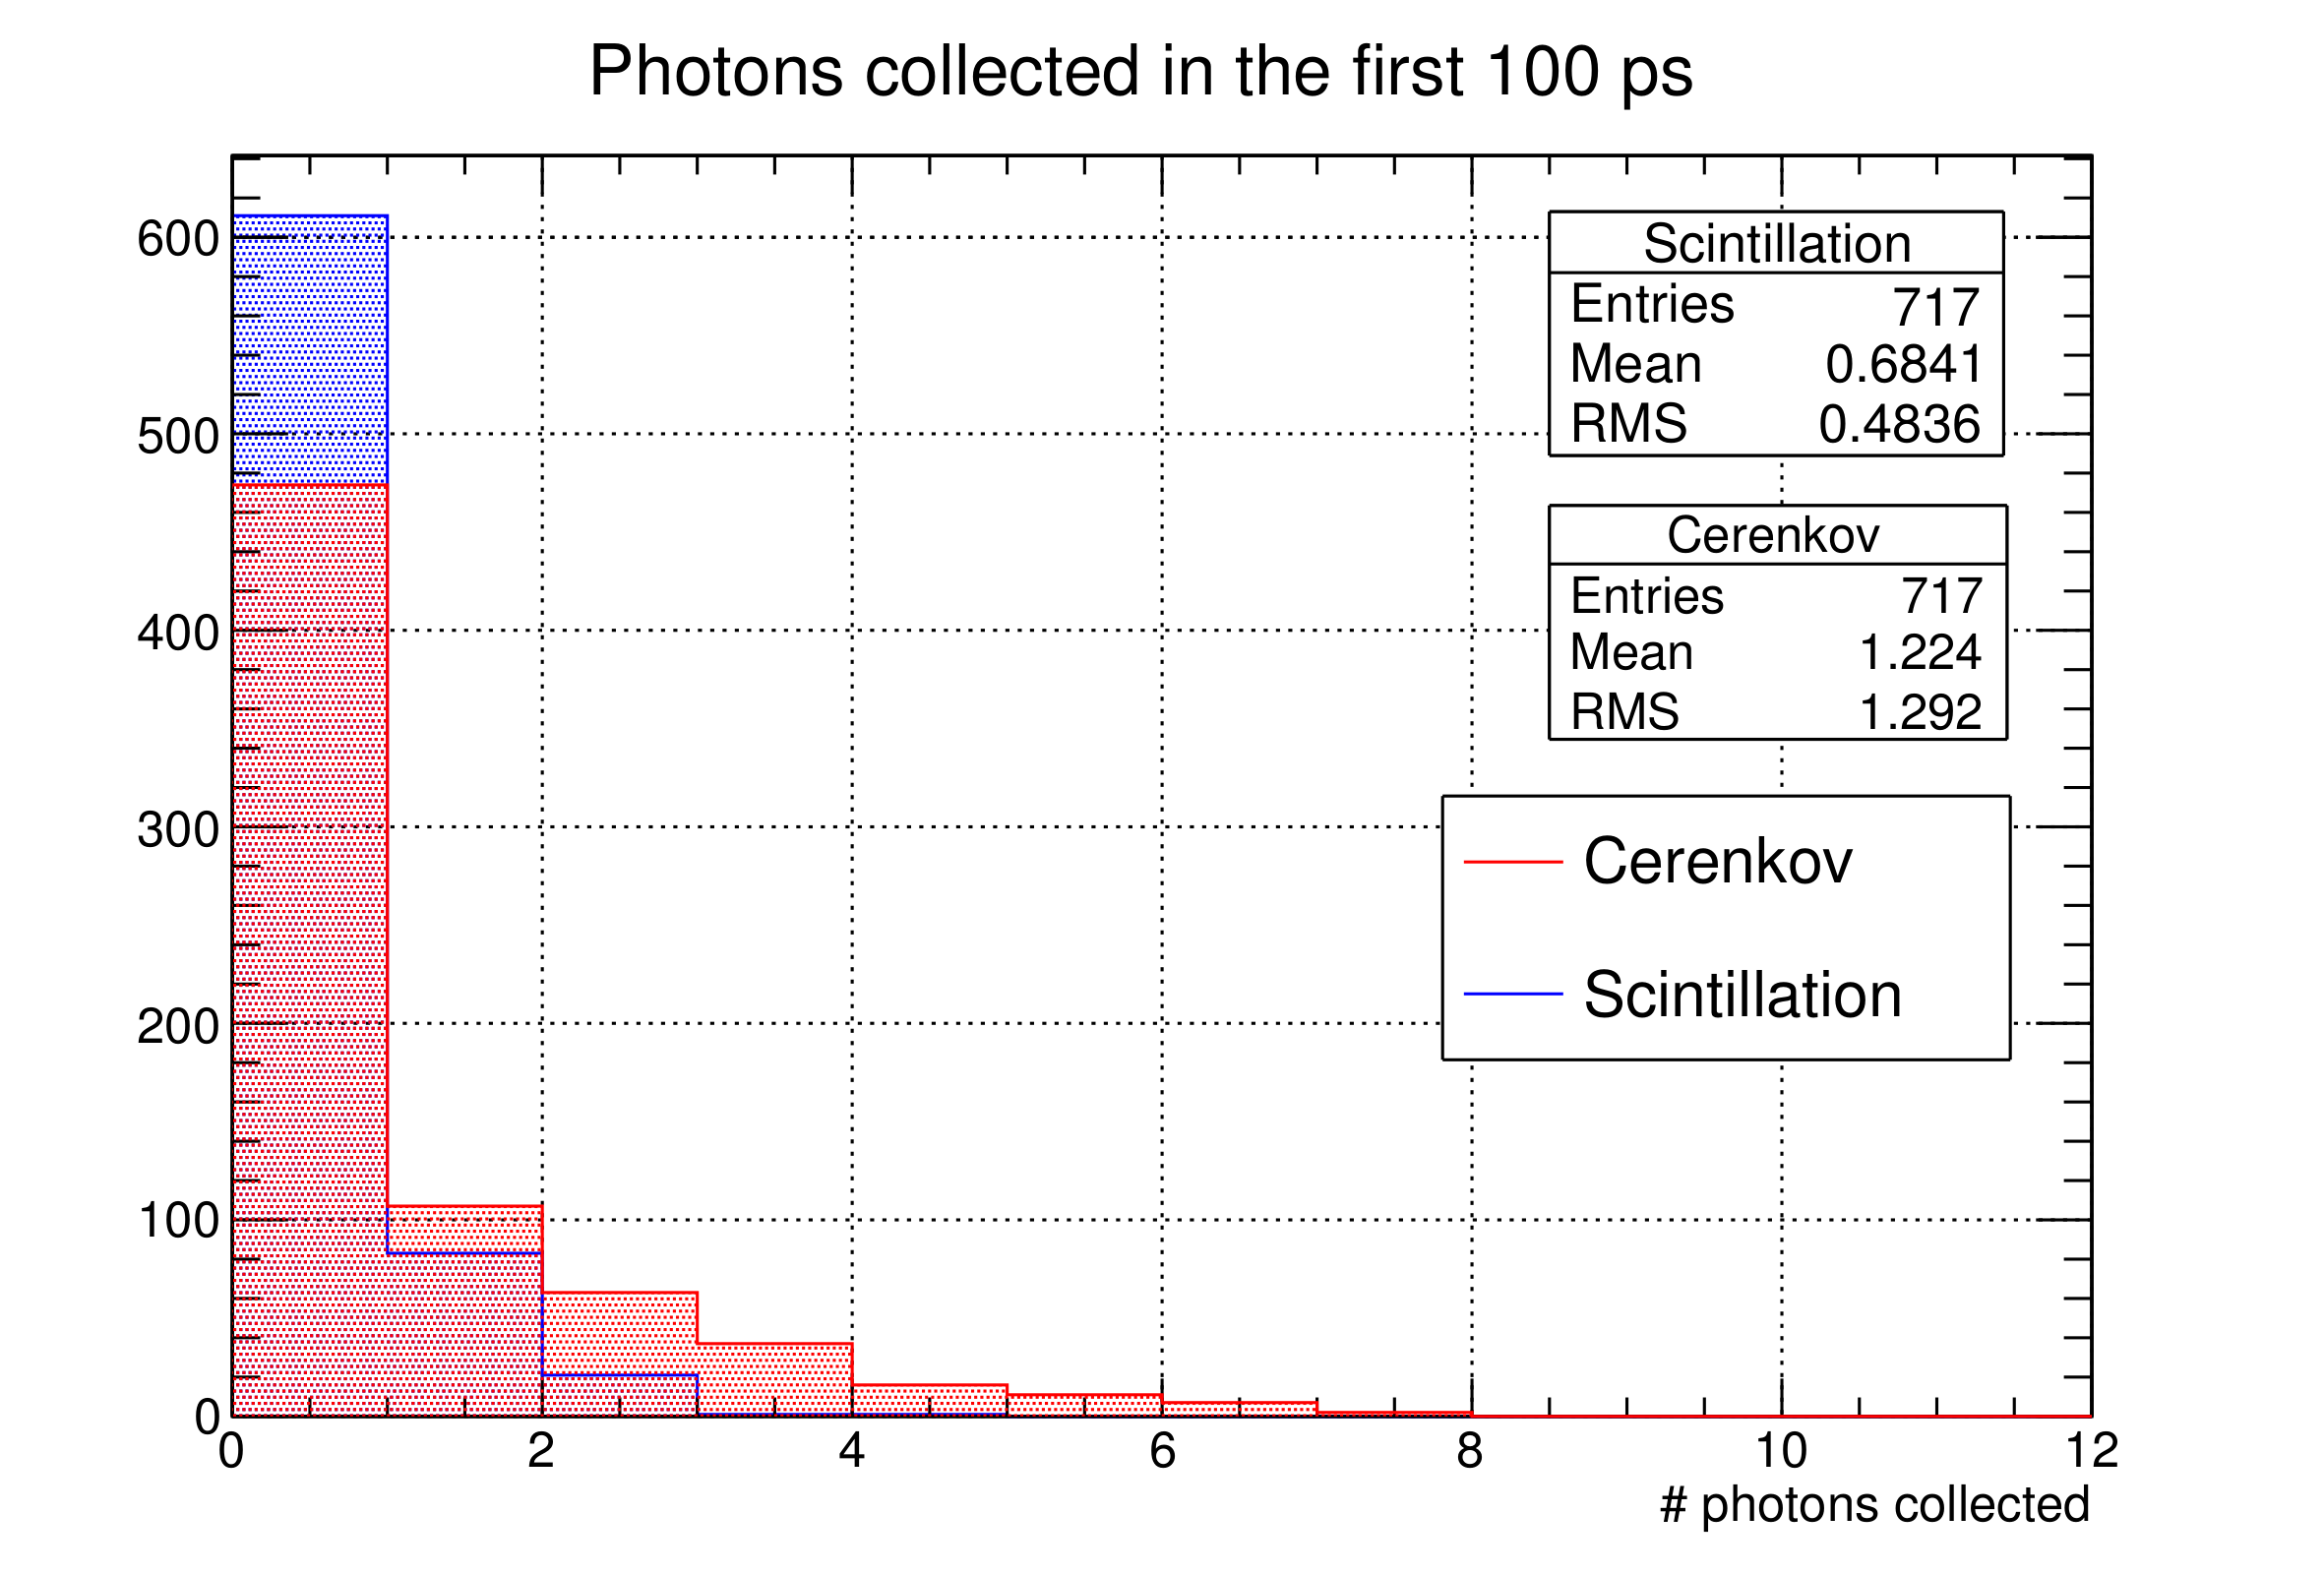
\includegraphics[width=10cm]{../Pictures/Chapter_5/cer_second_balance.png}
\end{center}
\caption[Scintillation/Cerenkov ratio in the first 100 ps]{The Cerenkov photons collected in the first 100 ps are comparable to the scintillation collection.}
\label{fig:time_ratio}
\end{figure}

\subsection{Rise time model}
The rise time model implemented in Geant4 is very simple, and given the energy deposition map in the crystal volume very similar to that of SLitrani. 
As soon as the program calls for energy deposition in a specific point, below the cut value set for the simulation, the scintillation process is called. 
At this point a bunch of isotropically distributed photons is produced, with the time profiles specified for the material.
All the parameters are defined at input: light yield (photons per MeV), energy resolution scale, scattering length, absorption length, index of refraction, fluorescence spectrum. 

In terms of timing, the LiverMore/Penelope libraries allow for reliable tracking down to 250 eV. This means that the time scale that divides this level of energy (tens of times higher than the band gap of heavy scintillators) to the recombination stage is included in the rise time parameters. Thus there is no model describing thermalization stage, that is all the chain of processes that leads electron hole pairs to recombine at luminescent centres. Attempts to include this stage in a simulation frame have been performed separately, see for example the work presented \cite{Vasiliev2013}.

As a consequence, simulations allow for good modelling of processes taking place above the ionization threshold and until the lower bound of multi scattering processes in low energy electromagnetic libraries. Moreover, as soon as the production of photons takes place with the parameters plugged in for the specific material in use, photons are tracked according to the optical characteristics of the material.

This happens for the two software packages, but SLitrani does not account for Cerenkov events for low energy neutral particles. As shown in figure \ref{fig:scint_cer} this events account for a large part of the rising edge of the signal, thus making Geant4 the ideal choice for simulations concerning timing.
\begin{figure}[htbp]
\begin{center}
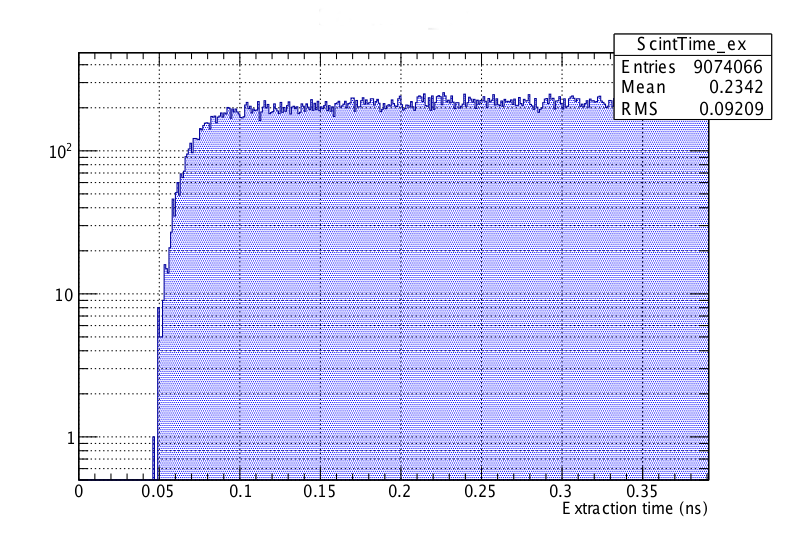
\includegraphics[width=10cm]{../Pictures/Chapter_5/scint_time_ex.png}
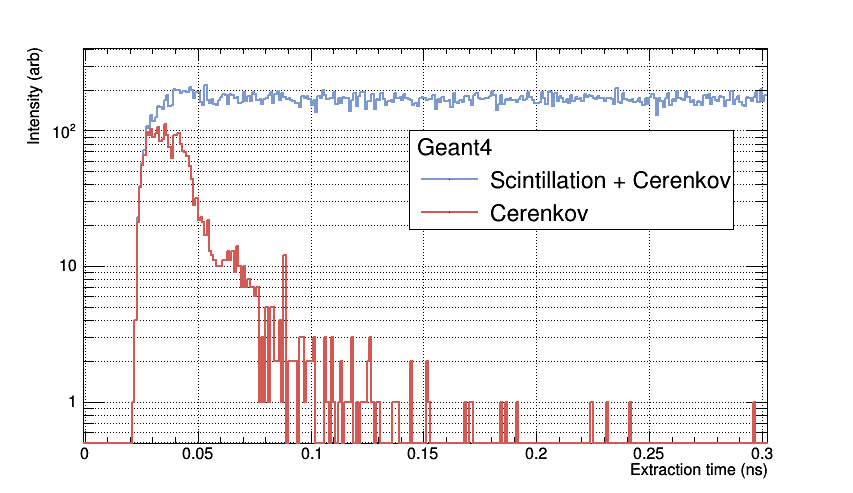
\includegraphics[width=10cm]{../Pictures/Chapter_5/sum_time_ex.png}
\end{center}
\caption[Simulated time profiles for LSO]{Simulated time profiles for LSO in SLitrani (top) and Geant4 (bottom)}
\label{fig:scint_cer}
\end{figure}

\subsection{Absorption and surface treatment}
Optical photons generated inside a crystal may undergo absorption processes (in the bulk or at a surface) and boundary interactions before being extracted or killed.
In order to test the differences between the software packages these events were tested with specified input parameters for absorption length and surface characteristics.
For absorption length optical photons were generated by a monochromatic source in the center of a very extended crystal. Reflection and refraction coefficients, on the other hand, where tested with a monochromatic beam of photons from the center of the crystal towards an interface with air.

The ratio of results obtained in SLitrani and Geant4, for LSO demonstrate perfect agreement between the two Monte Carlo software as shown in figure \ref{fig:abs}, both for Fresnel interaction and absorption processes. The parameters for the simulations were extracted with the procedure described in the next section.
\begin{figure}[htbp]
\begin{center}
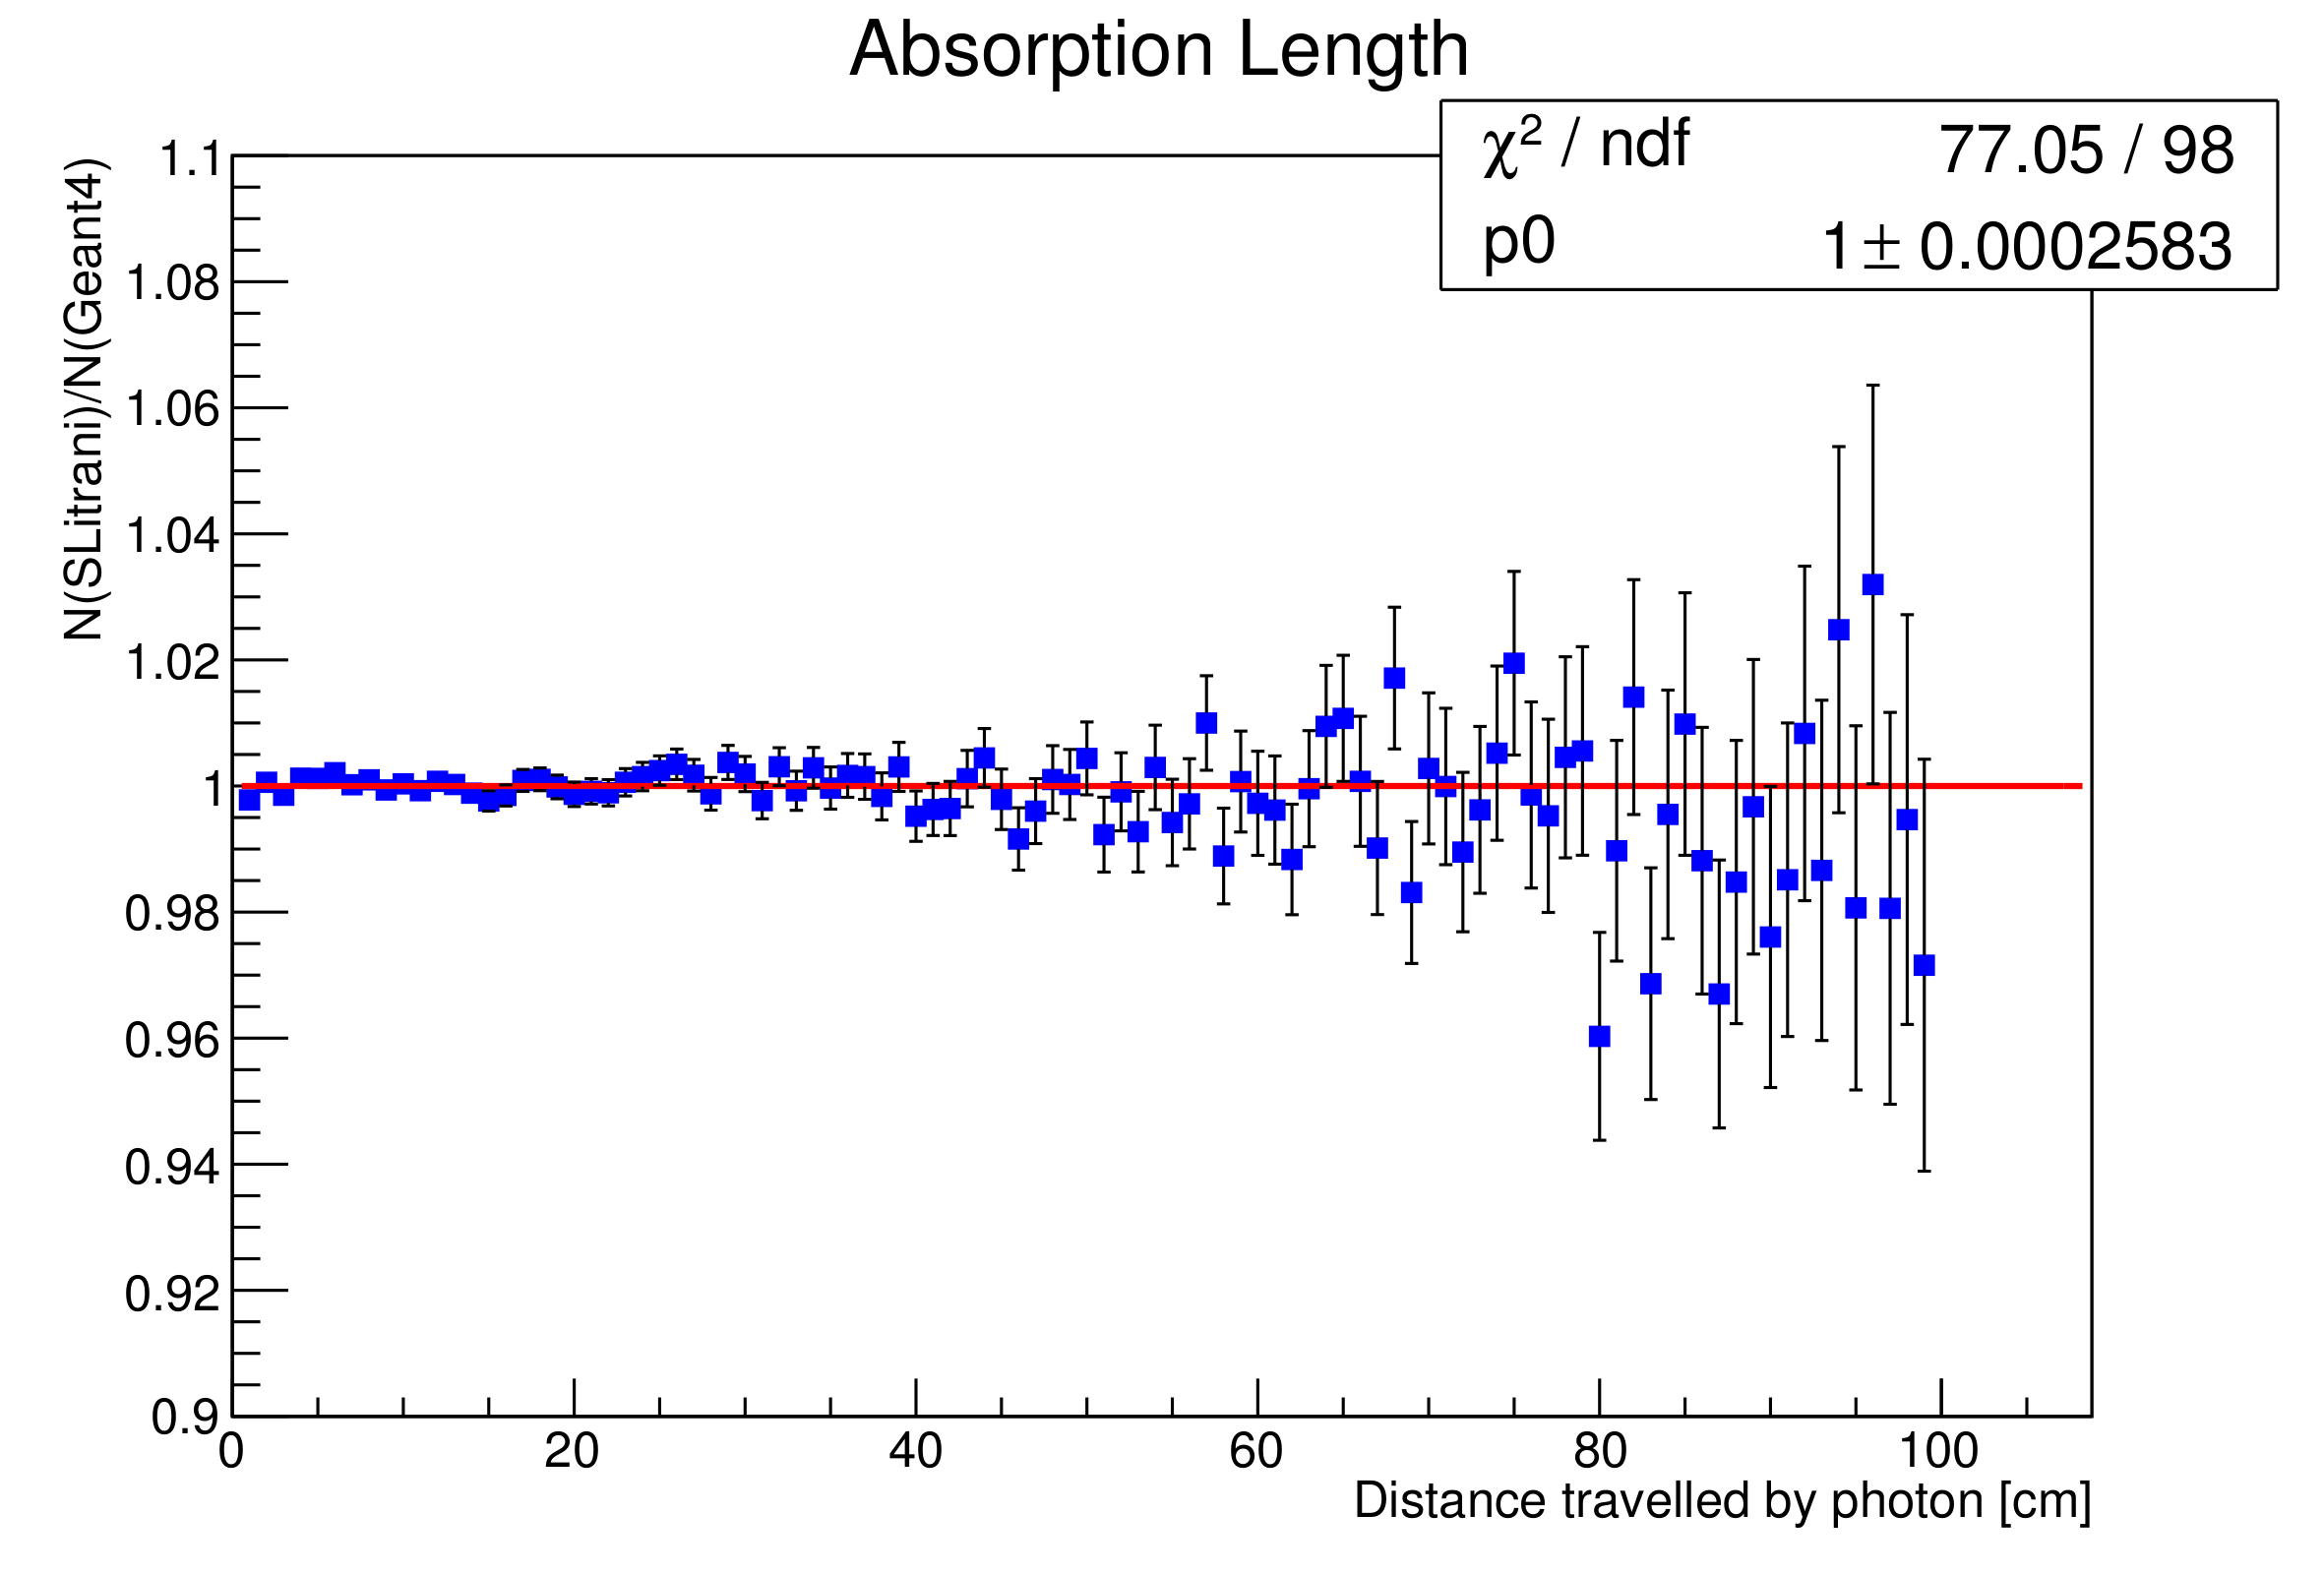
\includegraphics[width=10cm]{../Pictures/Chapter_5/abs.png}
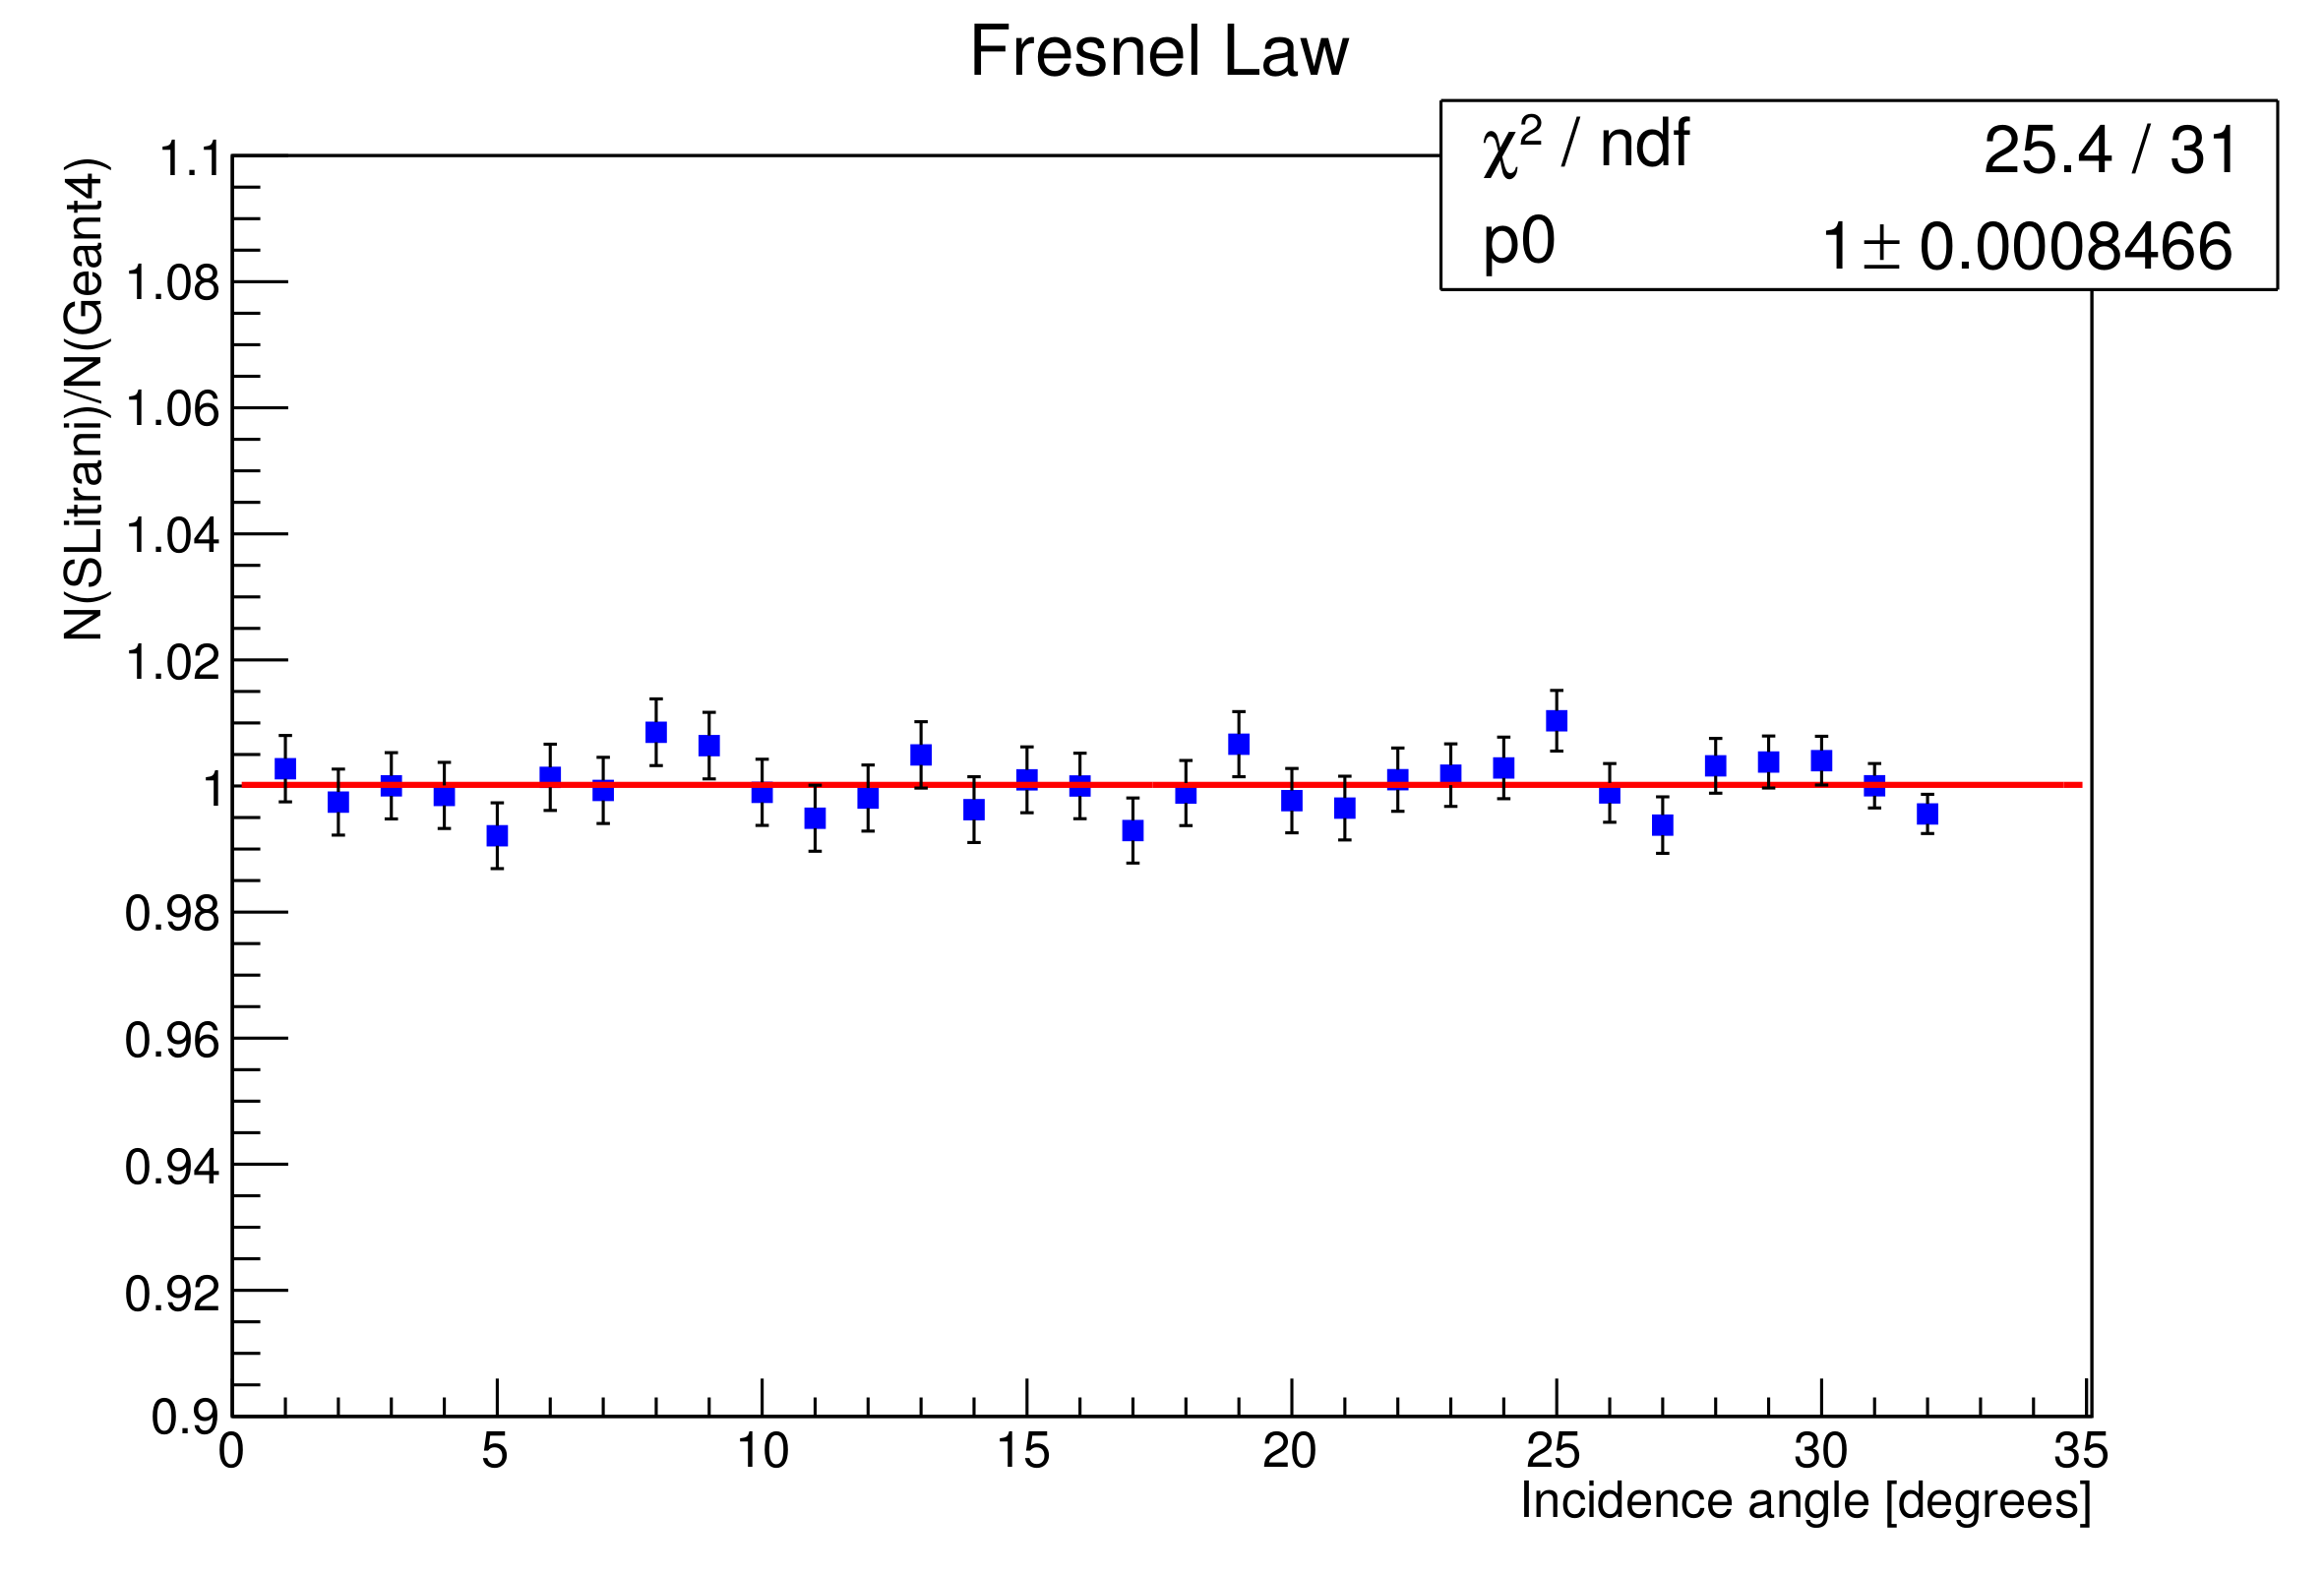
\includegraphics[width=10cm]{../Pictures/Chapter_5/fresnel.png}
\end{center}
\caption[Geant4 SLitrani absorption and reflection]{Ratio of photon absorbed in the simulation configuration (top) and ratio of photons reflected at different angles (bottom).}
\label{fig:abs}
\end{figure}

In order to test the models for boundary interaction with wrappings or coatings, the absorption of photons at boundary interface was tested by firing a monochromatic beam of photons towards the surface boundary and varying the incidence angle. The results obtained for the two software are shown in figure \ref{fig:surface}.
A significant difference is found for diffusive wrappings, with SLitrani showing an higher absorption rate for high incidence angles. This is due to the different modelization of the absorption  at boundaries. In fact, Geant4 determines the reflection based on the extracted value of the facet before the tilting considering an average value, while SLitrani does it for every angle.
\begin{figure}[htbp]
\begin{center}
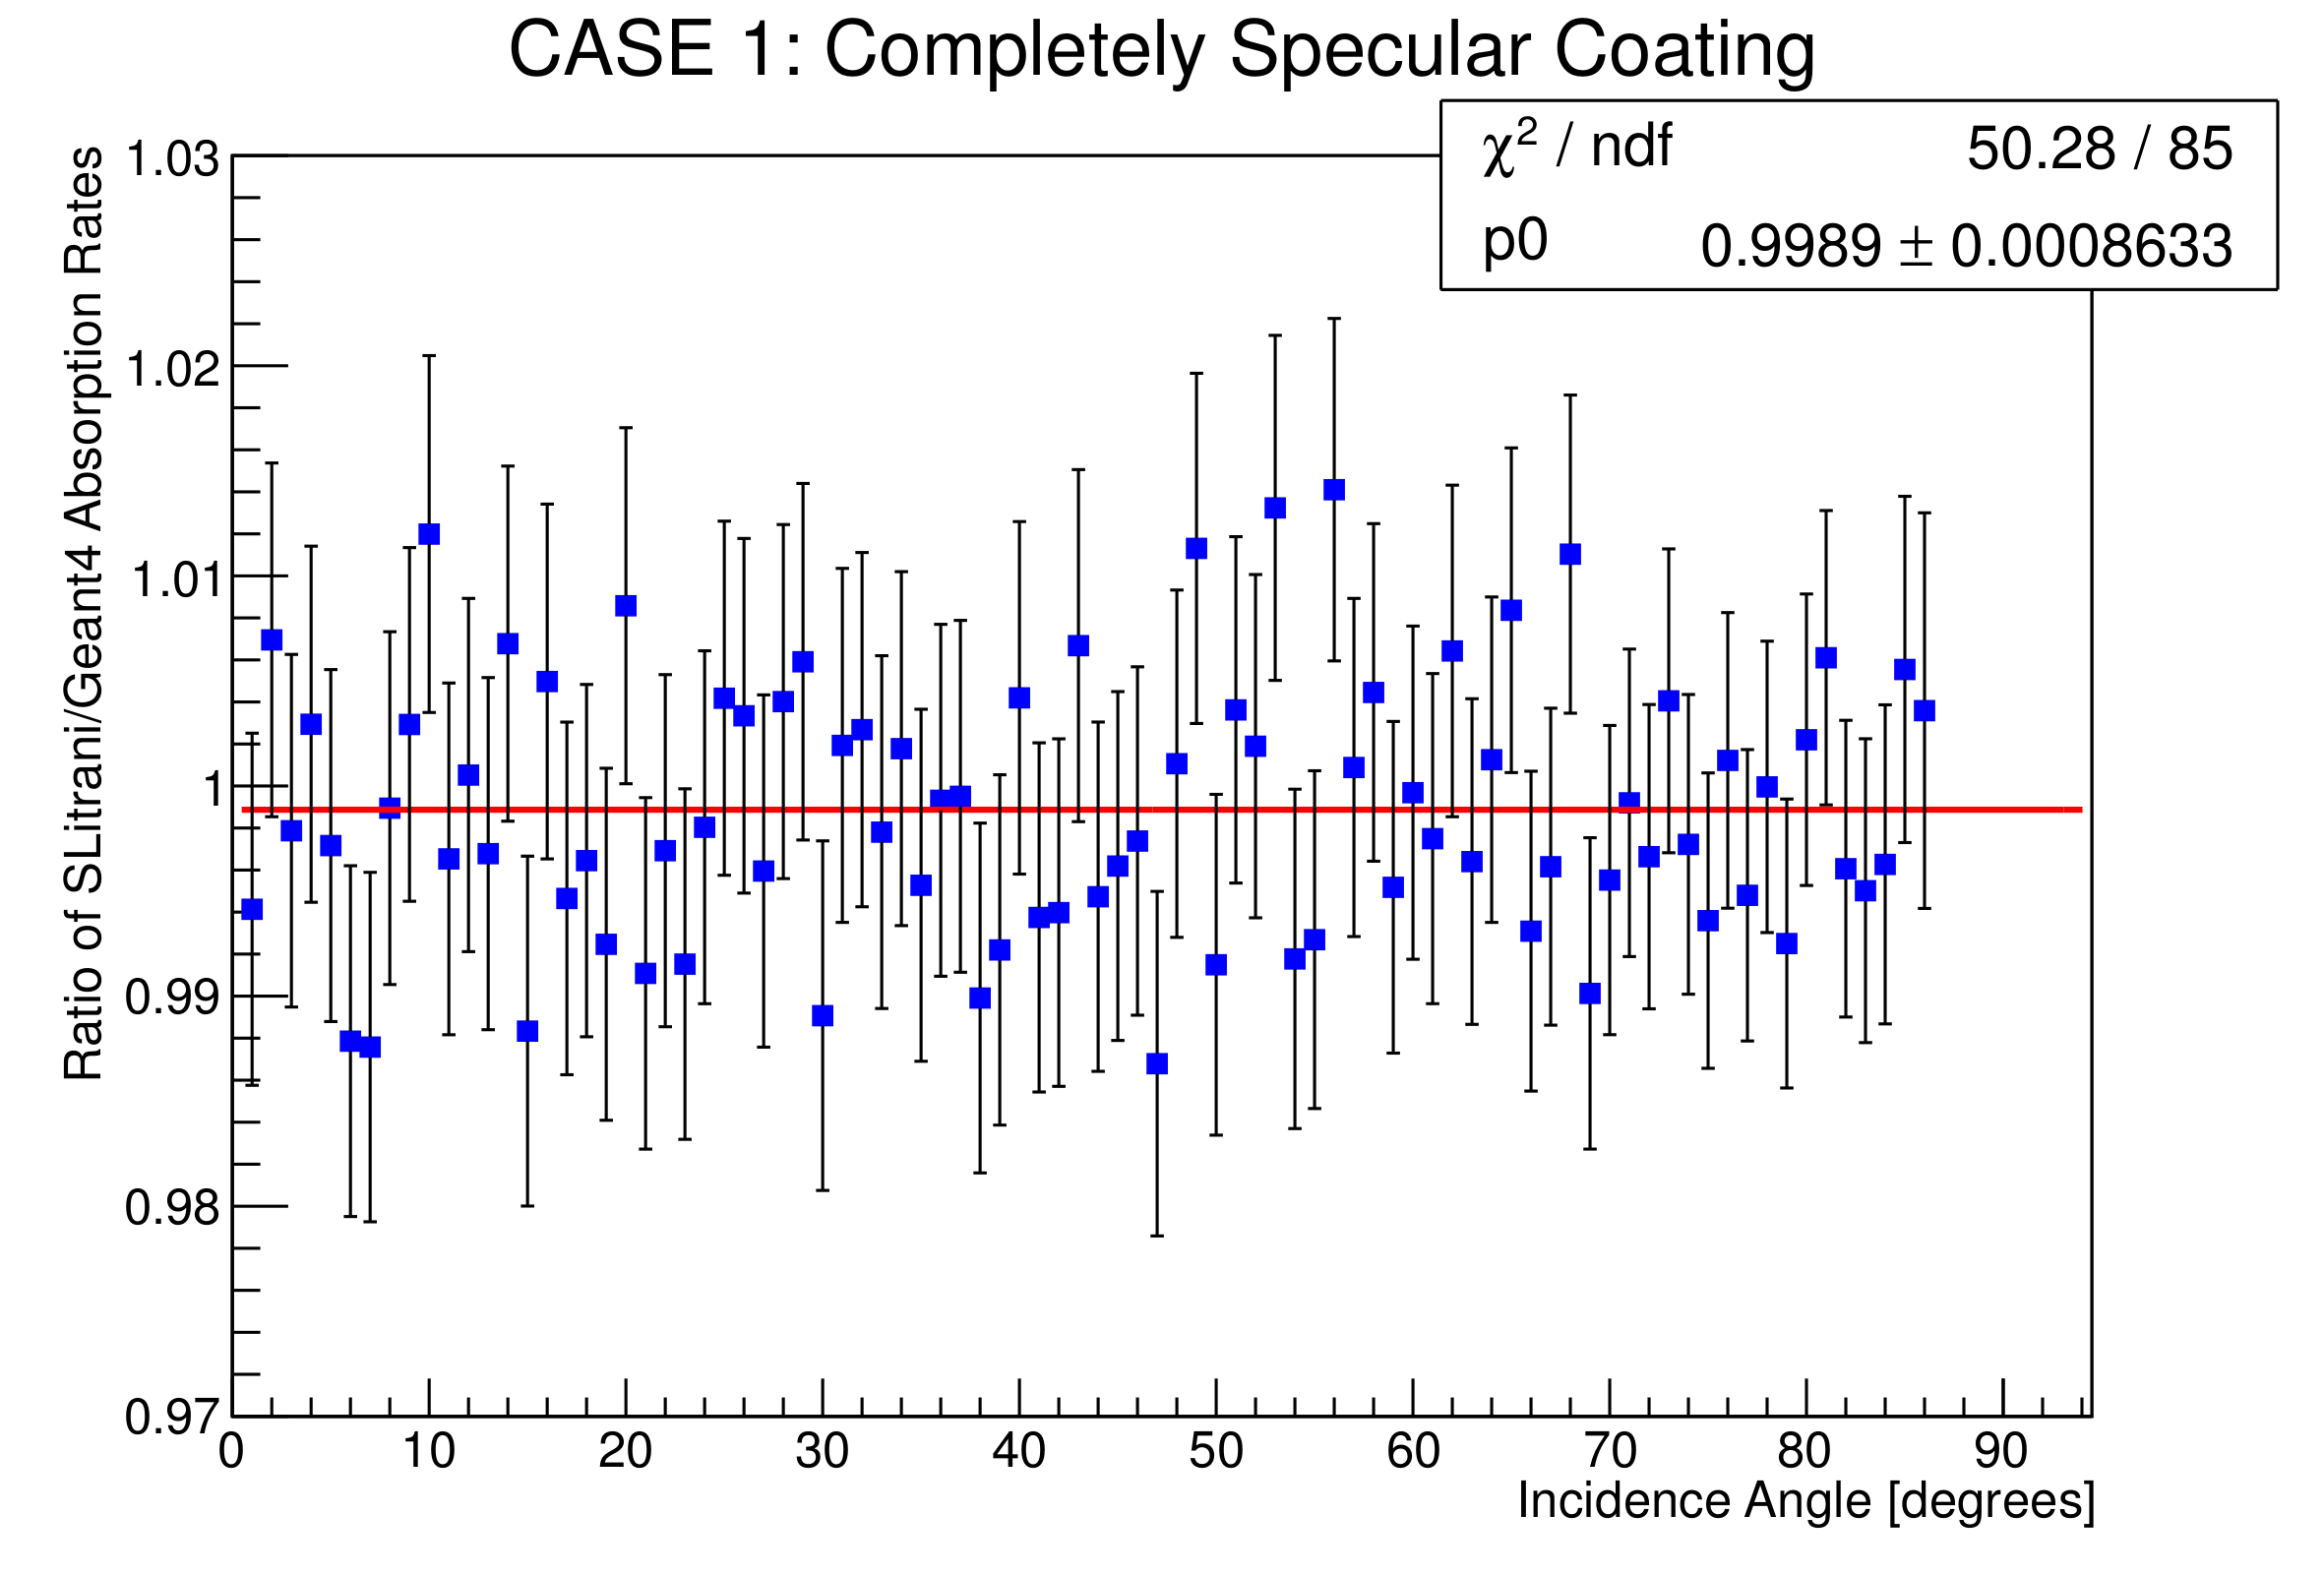
\includegraphics[width=10cm]{../Pictures/Chapter_5/specular.png}
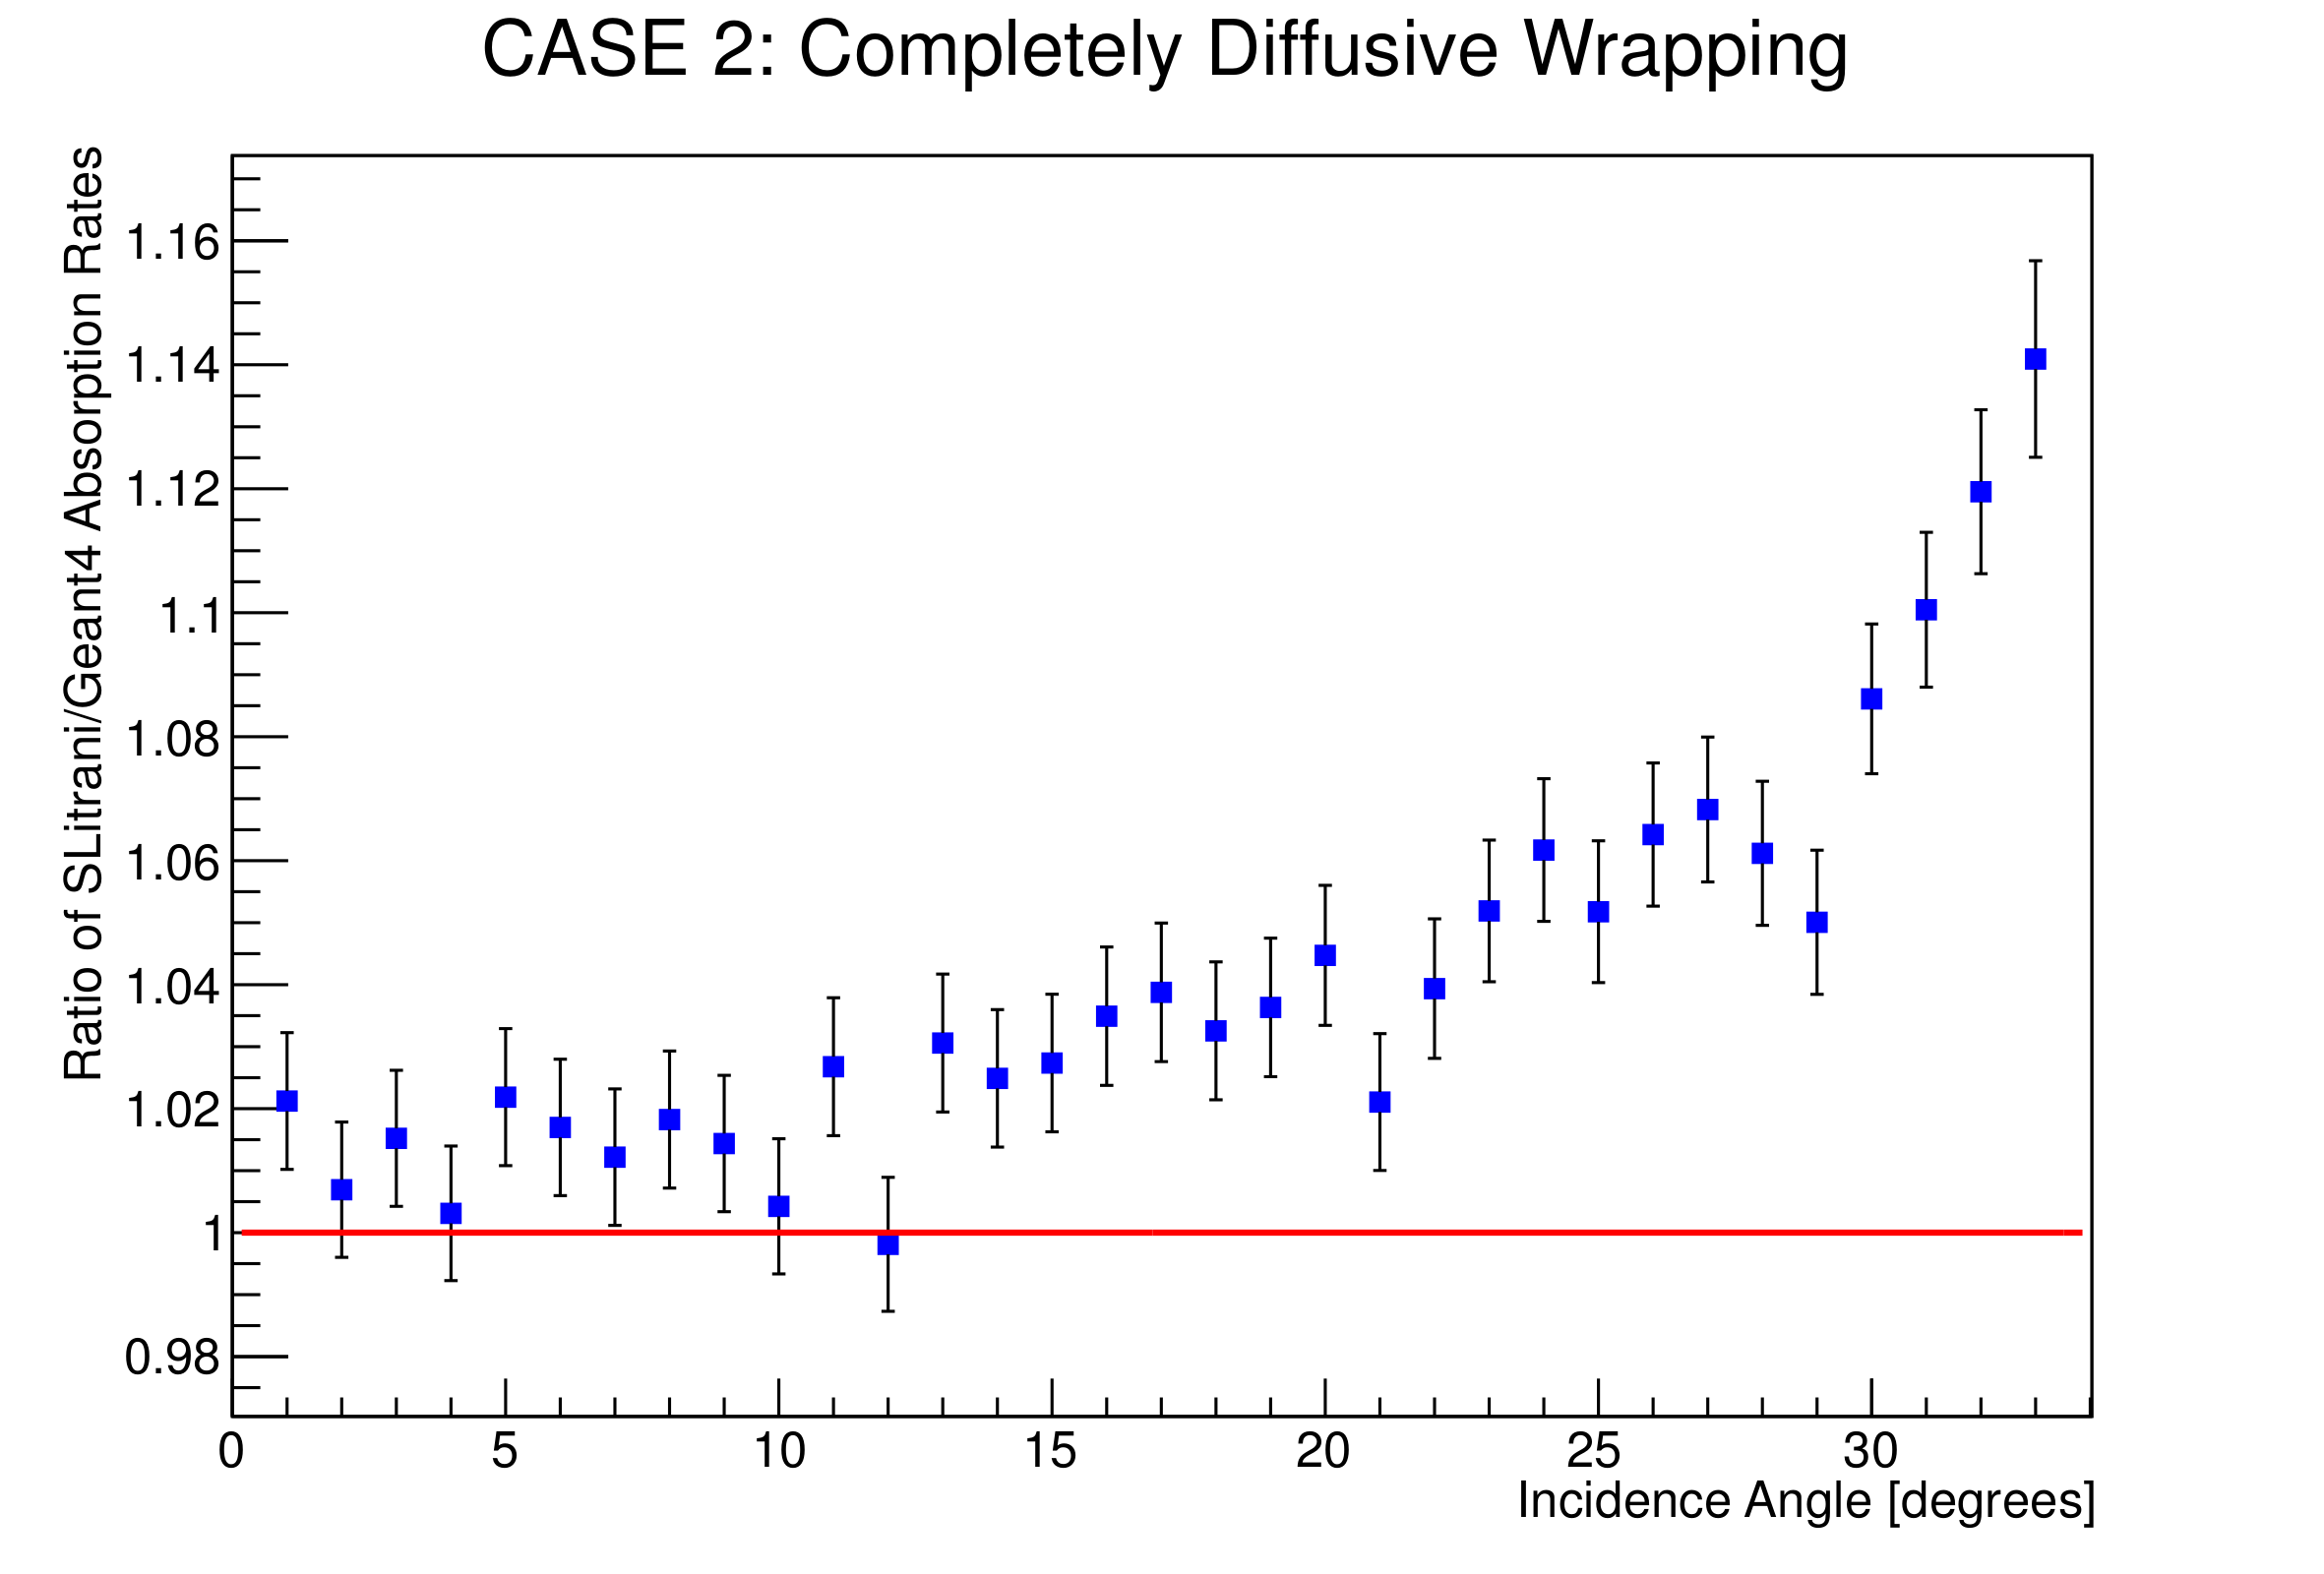
\includegraphics[width=10cm]{../Pictures/Chapter_5/diffusive.png}
\end{center}
\caption[Geant4 SLitrani specular and diffusive reflection]{Ratio of photons reflected for completely specular coating (top) and completely diffusive wrapping (bottom)}
\label{fig:surface}
\end{figure}

In order to evaluate the photon extraction efficiency in a realistic setup, a LSO crystal was simulated with an internal isotropic photon source, with a glass sensor placed with air gap from on of the exit faces.
Keeping a fixed crystal length (20 mm) while varying transverse section (from 0.56 mm$^{2}$ to 16 cm$^{2}$), the difference in the software packages were assessed for different surface states (wrapping, coating, depolishment) and crystal coupling to the detector (air and optical grease).
The results obtained for Teflon wrapping as a completely diffusive material are shown in figure \ref{fig:dimensions}.
As already inferable form the results in figure \ref{fig:surface}, a significant difference in photon extraction efficiency is found for small crystals.
It is possible to conclude that as the crystal section decreases, more bounces on the lateral faces are necessary for extraction. As SLitrani considers a higher absorption probability on the wrapping a discrepancy is measured.
\begin{figure}[htbp]
\begin{center}
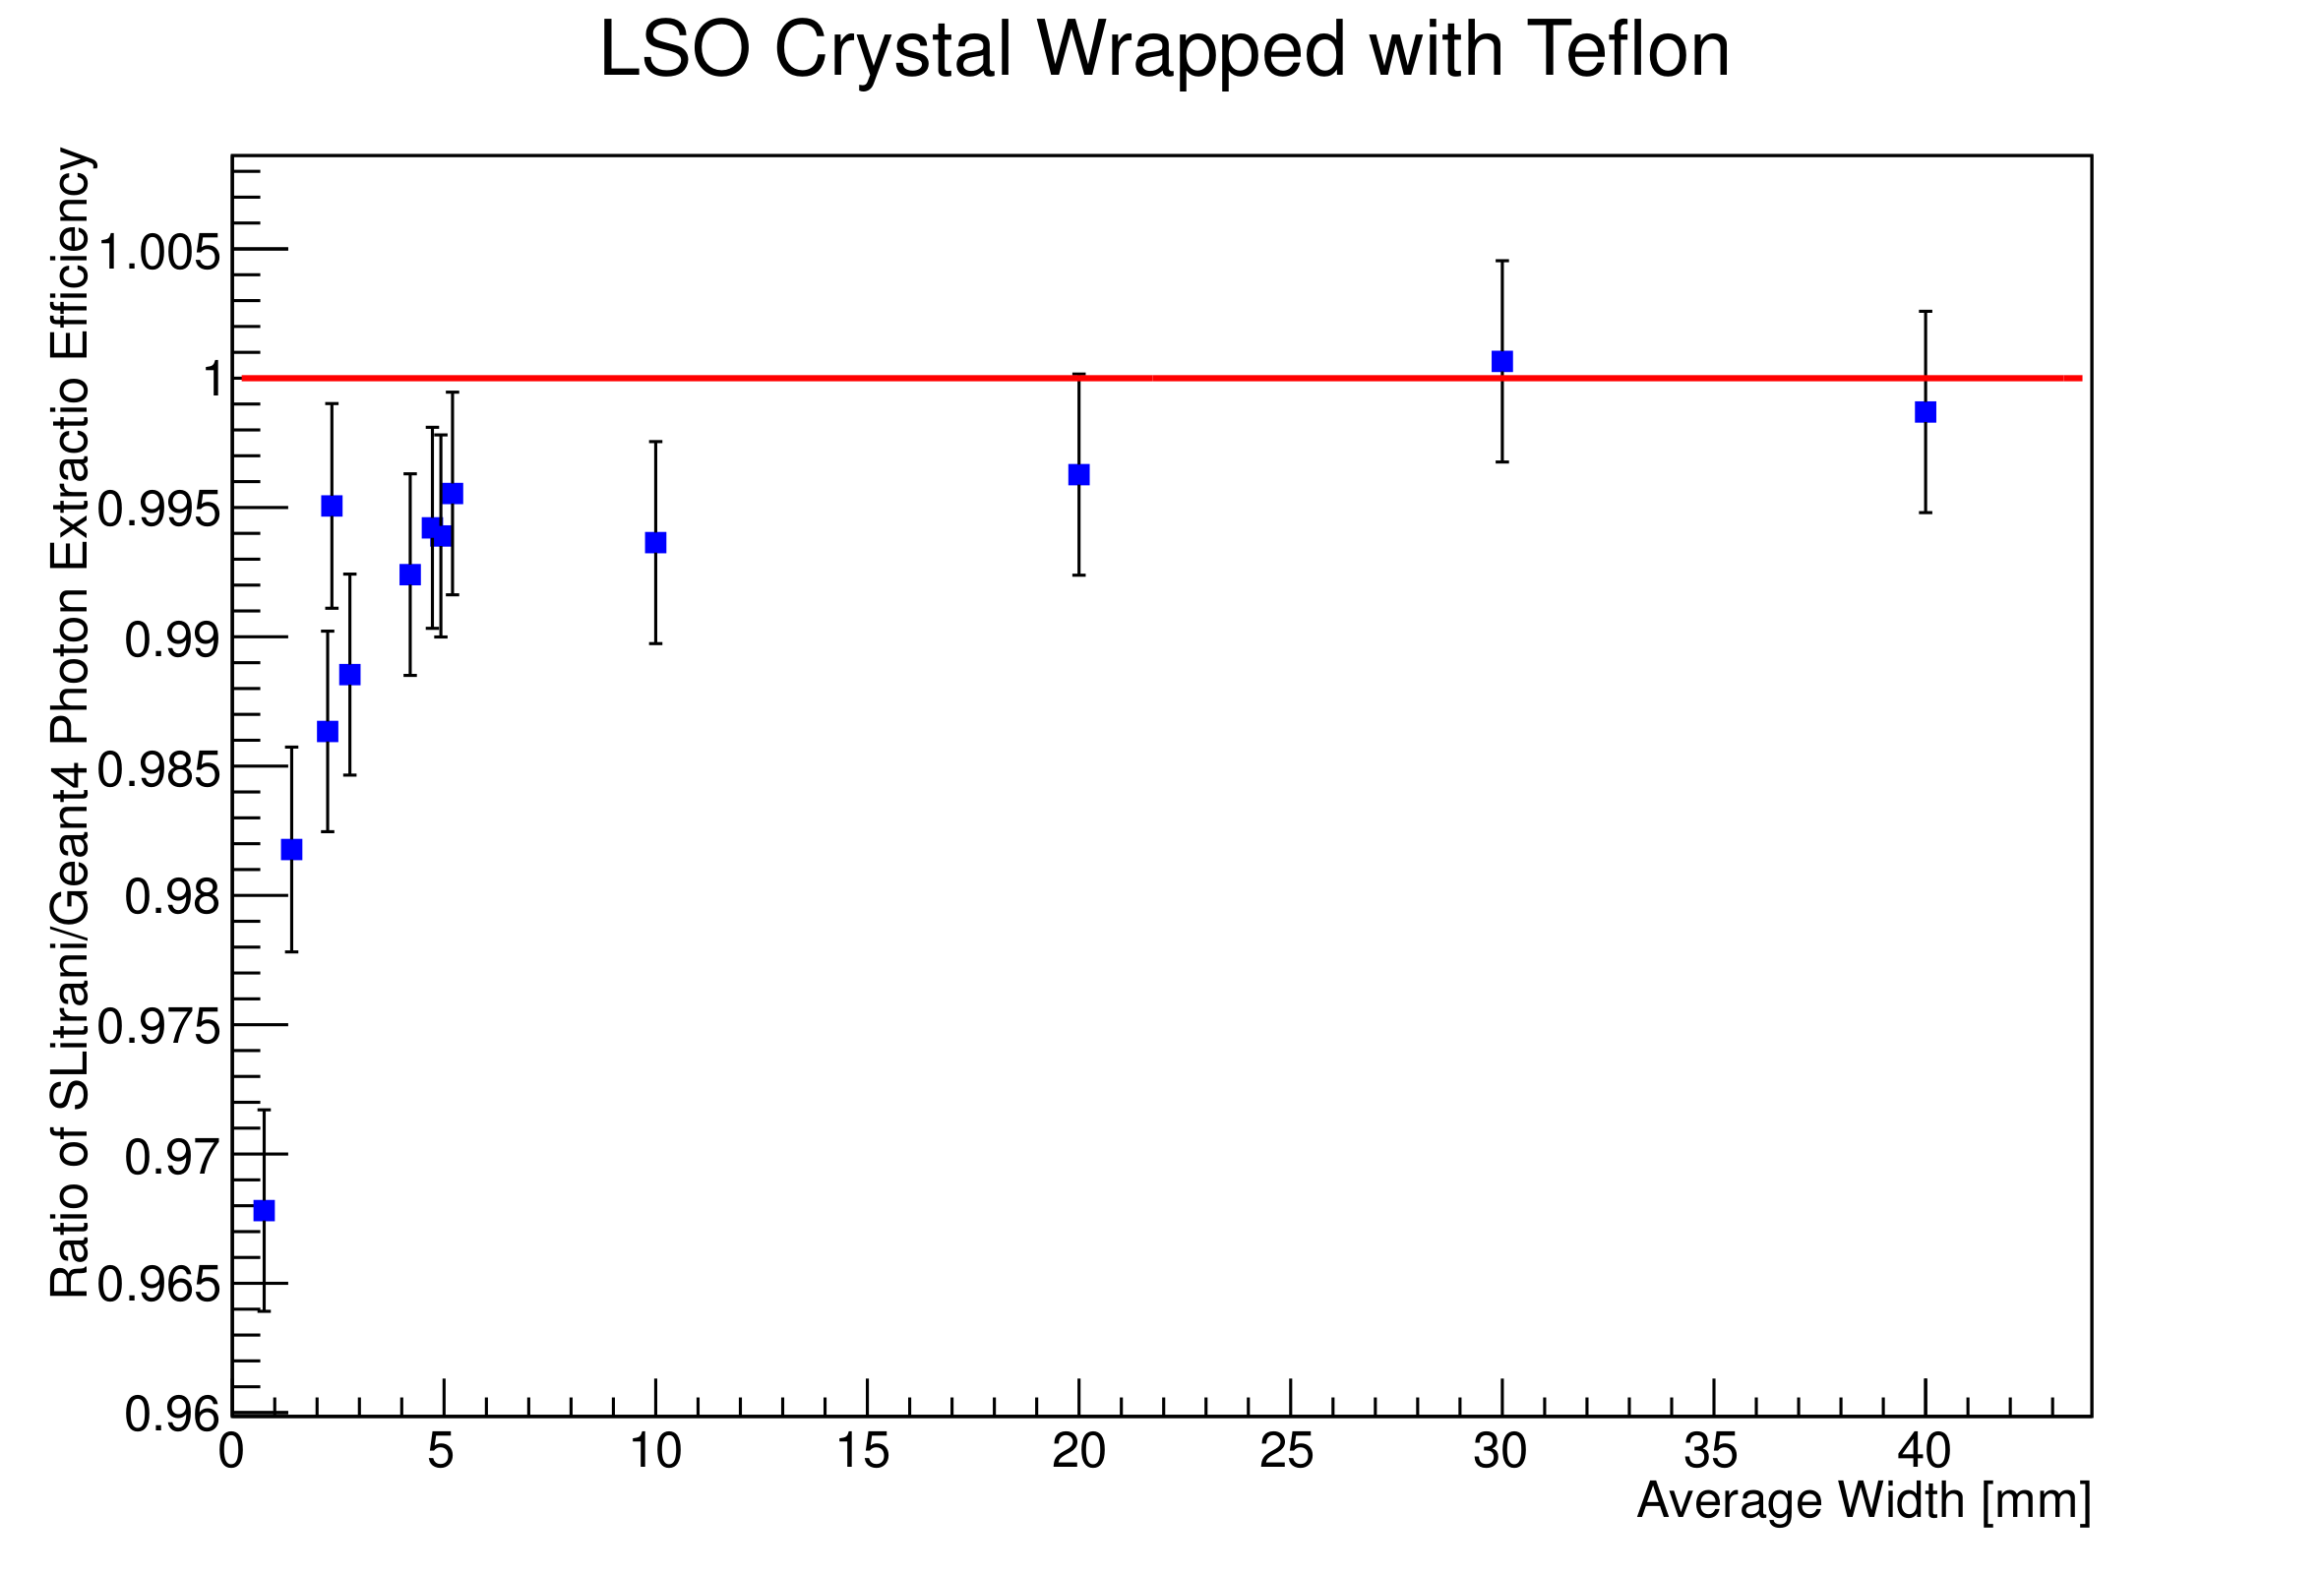
\includegraphics[width=10cm]{../Pictures/Chapter_5/size_LY_variation.png}
\end{center}
\caption[Geant4 SLitrani size ratio variation]{Ratio of photons extracted for different aspect ratio of the crystal simulated.}
\label{fig:dimensions}
\end{figure}
This results, though, seems to back the idea that a satisfying model for boundary interaction is still lacking. 

In fact, as a preliminary comparison with experimental data, the values measured in the study \cite{Kris2012} were considered, since full access to the experimental setup and materials was possible. 
The comparison was performed on the gain in the extraction coefficient obtained by coupling the crystal to a PMT with optical grease and by wrapping it with Teflon.
The gain profile given by the grease was qualitatively reproduced, as shown in figure \ref{fig:gain}. The systematic difference is due to poor knowledge of the optical grease index of refraction. 
On the other hand, the gain profile due to the use of
Teflon wrapping, is significantly different between
experimental data and Monte Carlo simulations, as shown in figure \ref{fig:gain}.
\begin{figure}[htbp]
\begin{center}
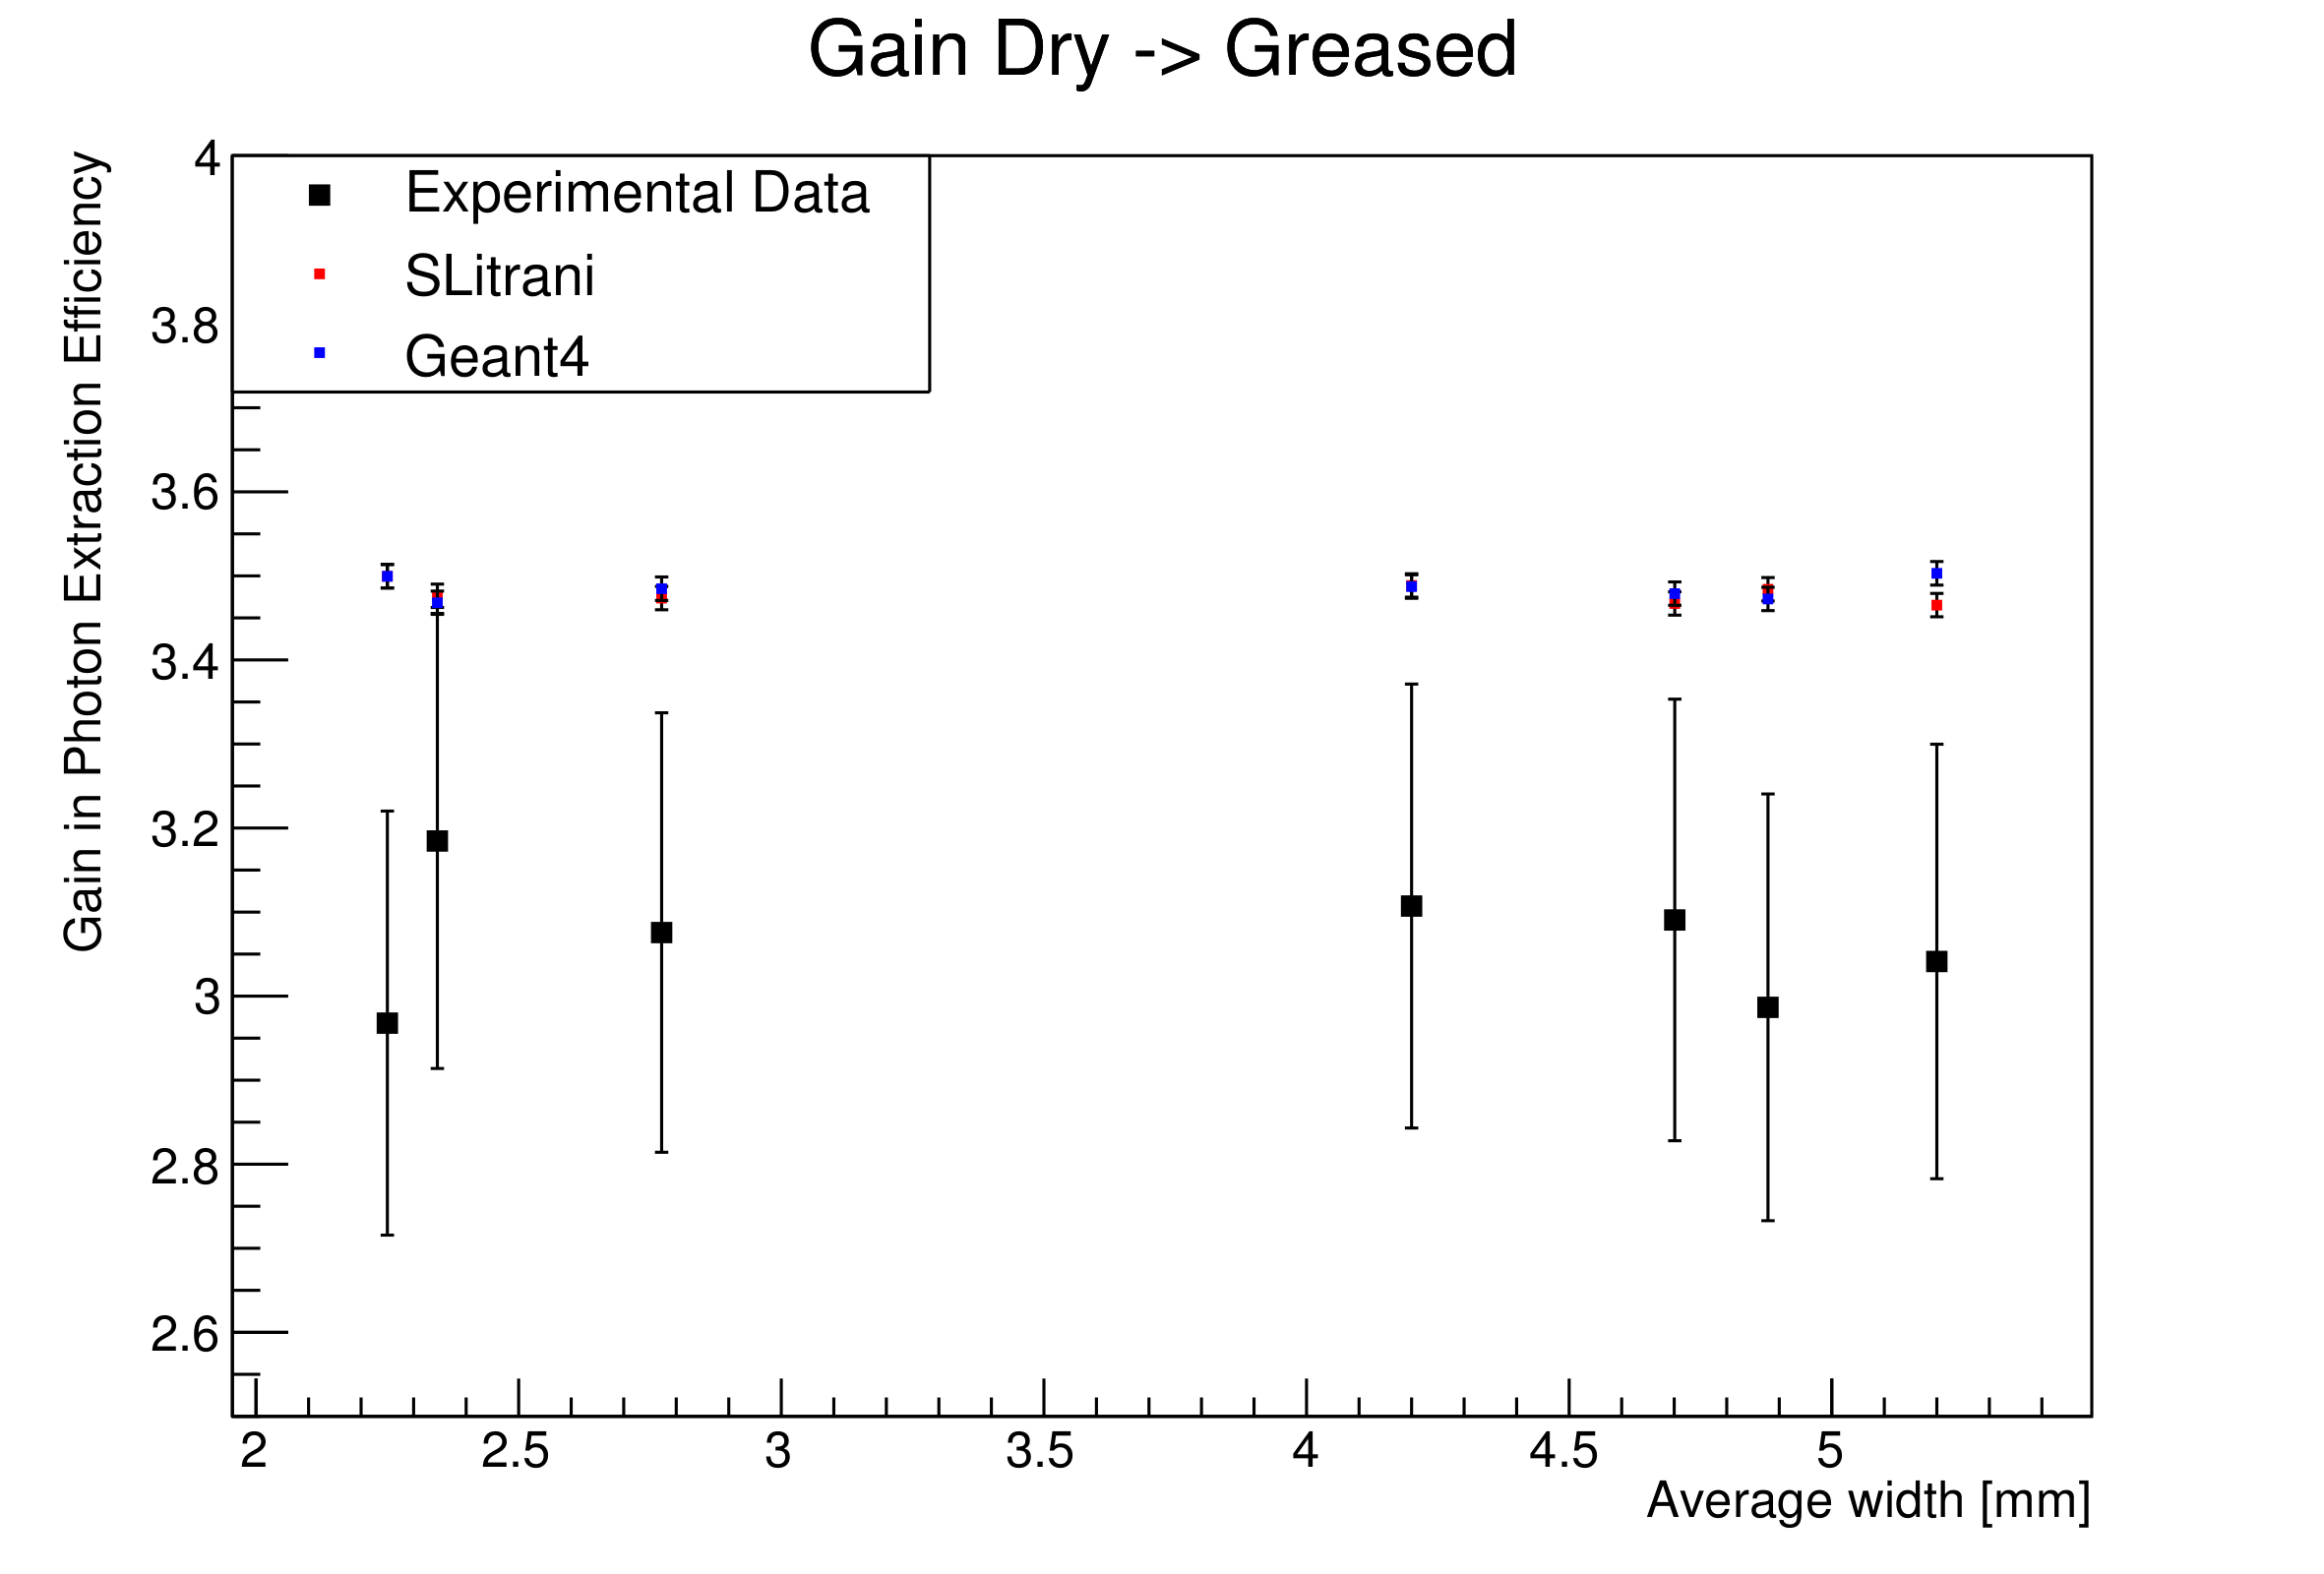
\includegraphics[width=10cm]{../Pictures/Chapter_5/gain_grease.png}
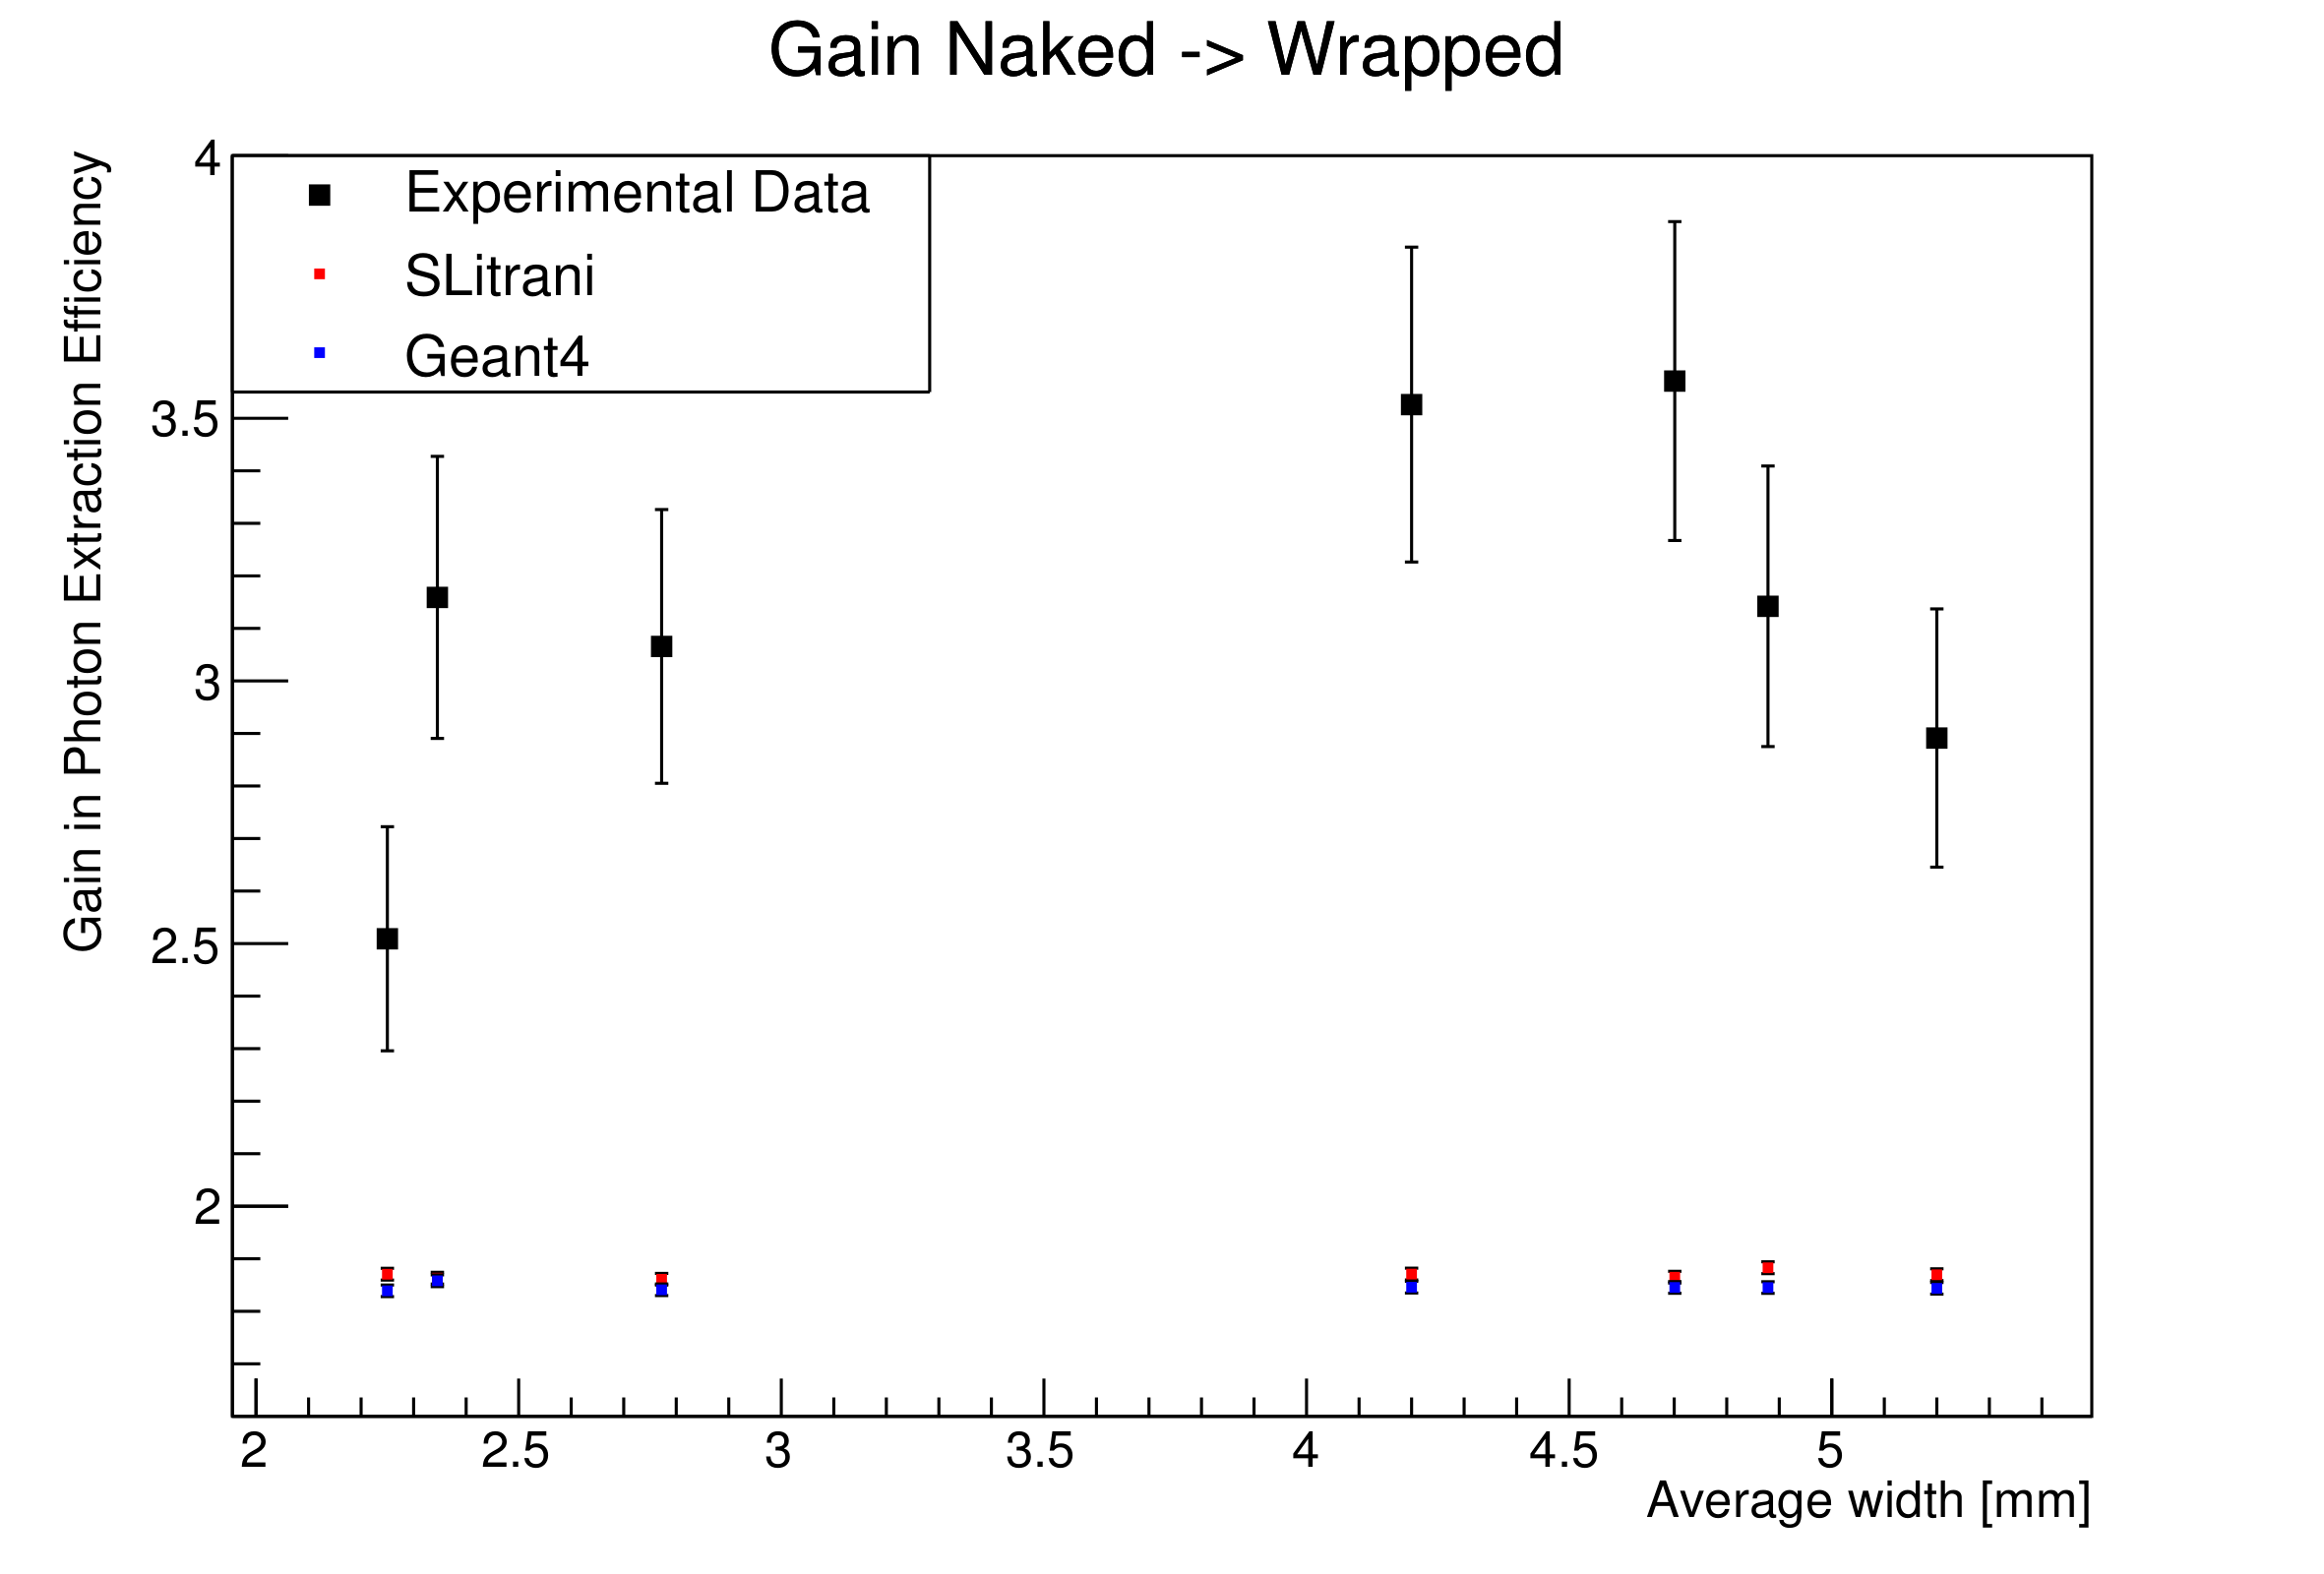
\includegraphics[width=10cm]{../Pictures/Chapter_5/wrap_gain.png}
\end{center}
\caption[Geant4 SLitrani gain profiles]{Gain profile for the two software with respect to the measured data for grease coupling (left) and Teflon wrapping (right).}
\label{fig:gain}
\end{figure}
Given this poor modelling of surface interaction we relied mainly on the simplest models available for the software packages, that is polished surface and Lambertian wrapping. No significant inferences can be made on light extraction, so timing simulation were tuned on parameters measured separately.

For the analysis of the measured data, we will make use of Geant4 in order to disentangle the elements contributing to signal formation in a scintillator system, since SLitrani does not offer the same processes in terms of photon production.
These three stages will be considered as the main components of the rising edge: energy deposition above the ionisation threshold, thermalization phenomena, photon transportation.
\newpage
\section{Simulation input parameters}

It has emerged from the previous discussion that the time scales involved in the relaxation phases following a $\gamma$ event in a crystal, become relevant at the thermalization stage. This emerges also from simulation packages at the keV scale.
After photon production optical tracking inside the volumes takes place. The influence of this stage strongly depends on the size of the crystal, because scattering and absorption in the bulk start to importantly degrade the performance in terms of light collection.
In order to properly describe this chain of processes and disentangle the various contributions that lead to the resolution loss, it is thus necessary to measure the input parameters of the crystals.
% qui l elenco va fatto bene!
For what concerns refractive indices the values previously introduced from literature were considered, since no direct method was available to measure them.
Four parameters were then accessible to experimental assessment: light yield, excitation spectrum, emission spectrum, transmission curve.
The samples measured to obtain input parameters for Monte Carlo simulation were later characterized with $\gamma$ excitation as explained in chapter 9 (where possible the manufacturer is specified): 
\begin{itemize}
\item LuAG:Ce (0.13$\%$ doping)
\item LYSO (Sipat)
\item LYSO (Proteus)
\item LSO:Ce,Ca 
\item LSO:Ce (CTI)
\item BGO
\item CeF$_{3}$
\end{itemize}
%spiegare qui bene i sample, da richiamare rapidamente in VUV!
\subsection{Fluorescence spectrum}
In order to analyse the timing profiles of crystals measured and plug in the correct parameters for simulations, 
the energy levels of the samples were investigated with a spectro fluorimeter.
\begin{figure}[htbp]
\begin{center}
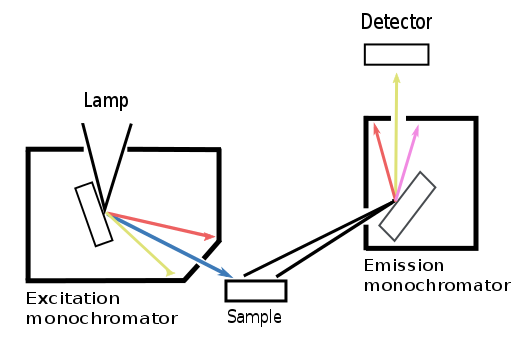
\includegraphics[width=8cm]{../Pictures/Chapter_5/fluo.png}
\end{center}
\caption[Spectro fluorimeter]{The setup used to measure excitation and emission spectra of the samples}
\label{fig:emission}
\end{figure}
 
As shown in figure \ref{fig:emission} a light source (tipically Xenon based) is used to generate photons over a certain range (200 nm - 800 nm) and two monochromators allow to select both the excitation and the emission wavelengths. 
Given a certain excitation wavelength it is then possible to measure the emission spectrum of the sample considered.
It is also possible to select a certain wavelength of emission and measure the excitation spectrum of the same sample.
Emission and excitation spectra of a LYSO (Sipat) and a LuAG:Ce crystal are shown in figure \ref{fig:luag_lso}.
The LSO, LGSO, LSO:Ce,Ca crystals do not qualitatively differ in terms of emission and excitation from the sample shown. 
The large bands are due to relevant electron-phonon coupling at higher temperatures.
The excitation spectra for the Cerium doped samples show the absorption peaks at 300 nm and 350 nm, associated with the Cerium sites absorption presented in chapter 2. The 5d$\rightarrow$4f transition is responsible for the typical emission band of the Cerium doped LSO and LuAG crystals. 
A similar consideration can be made for CeF$_{3}$
In the case of LuAG:Ce only the Cerium emission is investigated since for UV emission the instrumentation is not optimised.

\begin{figure}[htbp]
\begin{center}
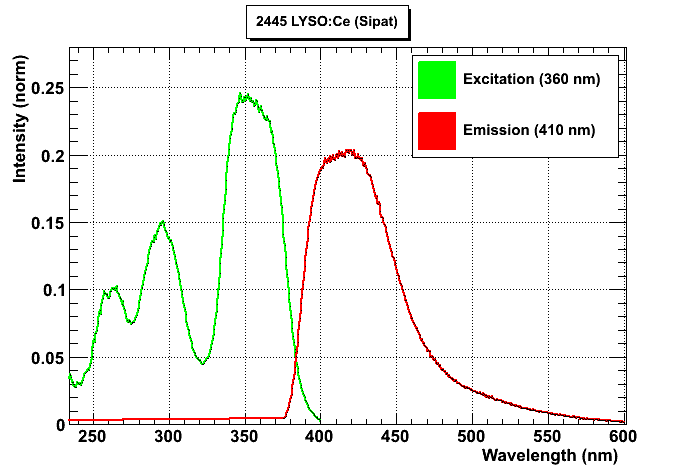
\includegraphics[width=7cm]{../Pictures/Chapter_5/LYSO_Sipat.png}
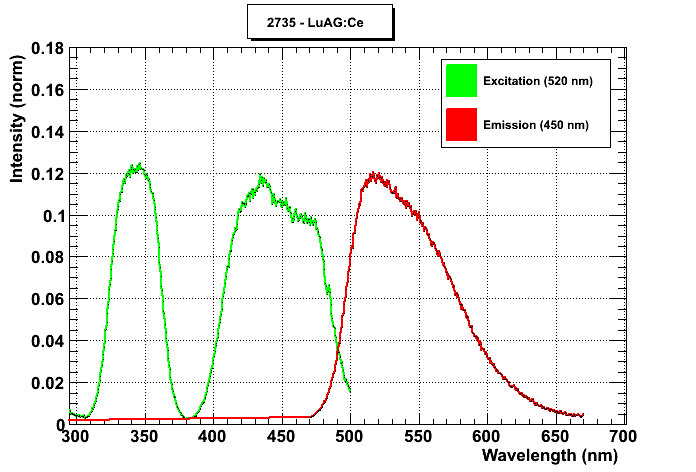
\includegraphics[width=7cm]{../Pictures/Chapter_5/LuAG_ce.png}
\end{center}
\caption[Sipat - LuAG excitation/emission]{Measured excitation and emission spectra for LYSO Sipat an LuAG: Ce}
\label{fig:luag_lso}
\end{figure}

The LuAG:Pr.excitation and emission spectra are shown in figure \ref{fig:luag_cef3}. The transition responsible is the 5d$\rightarrow$4f for Praseodymium sites.

\begin{figure}[htbp]
\begin{center}
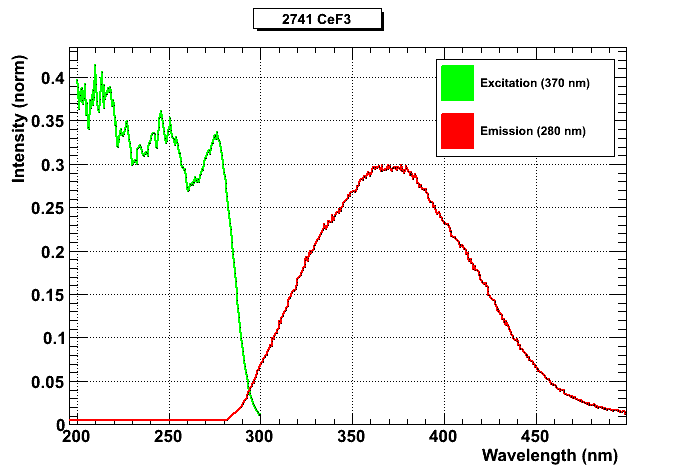
\includegraphics[width=7cm]{../Pictures/Chapter_5/cef3.png}
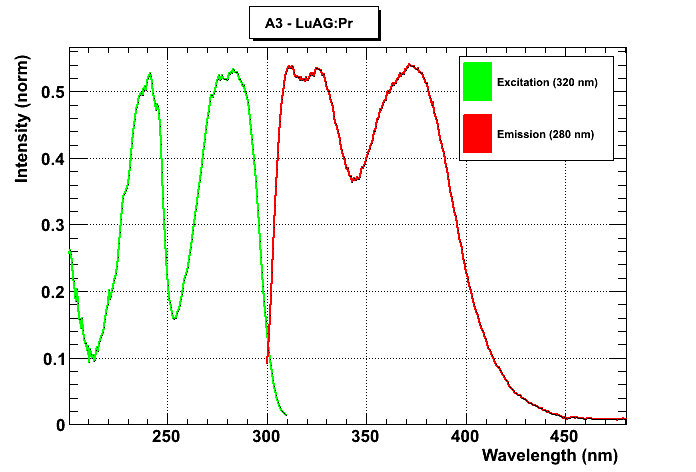
\includegraphics[width=7cm]{../Pictures/Chapter_5/LuAG_pr.png}
\end{center}
\caption[CeF$_{3}$ - LuAG excitation/emission]{Measured excitation and emission spectra for CeF$_{3}$ an LuAG: Pr}
\label{fig:luag_cef3}
\end{figure}

The BGO emission and excitation spectra are shown in figure \ref{fig:BGO}. The transition responsible is the Bi$^{3+}$ 6s6p(P$_{1}$)$\rightarrow$6s$^{2}$($^{1}$S$_{0}$).

\begin{figure}[htbp]
\begin{center}
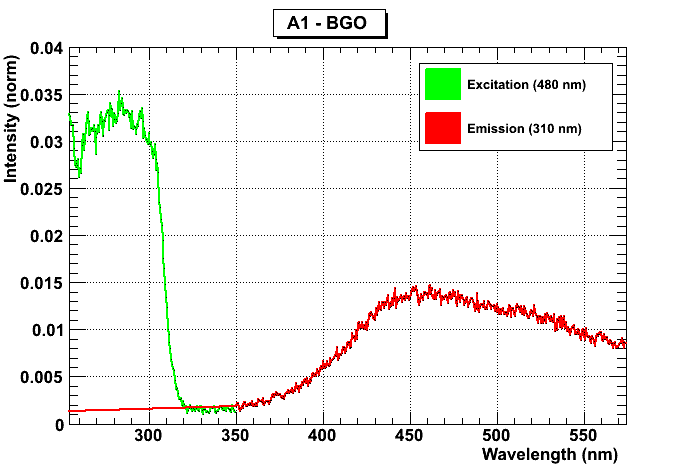
\includegraphics[width=8cm]{../Pictures/Chapter_5/BGO.png}
\end{center}
\caption[BGO excitation/emission]{Measured excitation and emission spectra for BGO}
\label{fig:BGO}
\end{figure}

\subsection{Optical transmission}
The next parameter analysed to extract the inputs for the simulations was the light transmission of the samples measured.
In order to extract meaningful values transmission spectra were measured for samples of different size, since the error is more significant when dealing with small pixels.
\begin{figure}[htbp]
\begin{center}
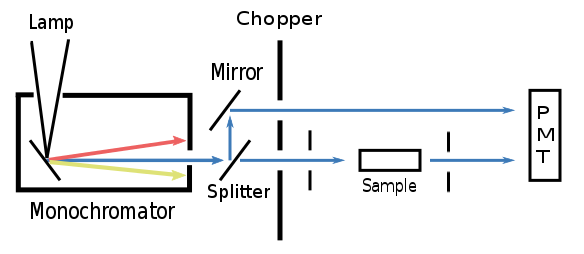
\includegraphics[width=8cm]{../Pictures/Chapter_5/trans.png}
\end{center}
\caption[Spectro photometer]{The setup used to measure the transmission curves of the samples}
\label{fig:transmission}
\end{figure}
The working principle is shown in figure \ref{fig:transmission}. The sample is crossed by a monochromatic beam of light. Before reaching the sample the beam is split, so that at the photodetector it is possible to compute the different intensities. This allows to measure the absorption length of the crystal at the different wavelengths.
The measurement determines the strength of the interactions of photons with the crystal. In general they will change the direction of diffusion, isotropically. Therefore, with a pinhole at the exit only non interacting the photons are coupled to the photo detector.

In the case of a perfect crystal, without impurities in the bulk and with perfect surface conditions the theoretical transmission at long wavelength still does not reach 100$\%$. This is due to Fresnel refraction, since at a boundary air-crystal the reflection coefficient is
\begin{equation}
r = \left( \frac{n_{1}-n_{2}}{n_{1}+n_{2}} \right) ^{2}
\end{equation}
where n$_{1}$ and n$_{2}$ are the indices of refraction of the two media. The transmission coefficient is defined as t $= 1-r$.
So this should be considered in the spectra presented below.
Including Fresnel effect is it possible to calculate the theoretical transmission as
\begin{equation}
T_{theory}=\frac{t^{2} \exp{\left( -L/\tau _{att} \right)}}{1-r^{2}\exp{\left( -L/\tau _{att} \right)}}
\end{equation}
where L is the length of the material and $\tau _{att}$ is the attenuation coefficient of the medium.
Starting from the transmission value measured, we can extract the attenuation values for simulation with the approximation
\begin{equation}
\frac{1}{\tau _{att}} = -\frac{1}{L} \log{\frac{(1-r)^{2}}{T}}
\end{equation}
where T is the measured transmission and r is the reflection coefficient.
Transmission spectra for the crystals measured are shown in figures \ref{fig:luag_lso_trans} and \ref{fig:luag_lso_trans}.
\begin{figure}[htbp]
\begin{center}
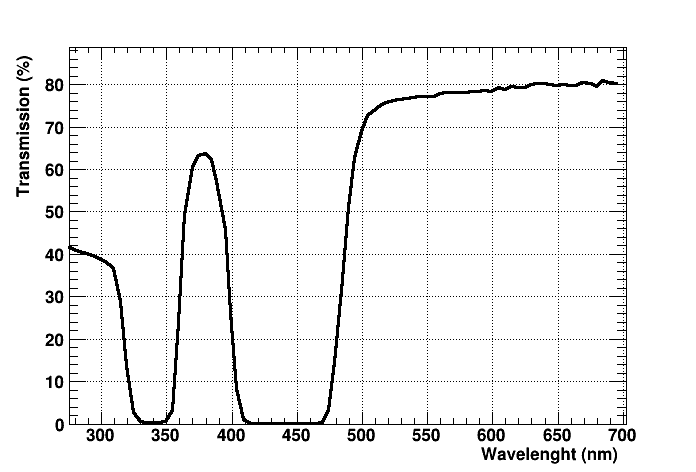
\includegraphics[width=7cm]{../Pictures/Chapter_5/trans_luag.png}
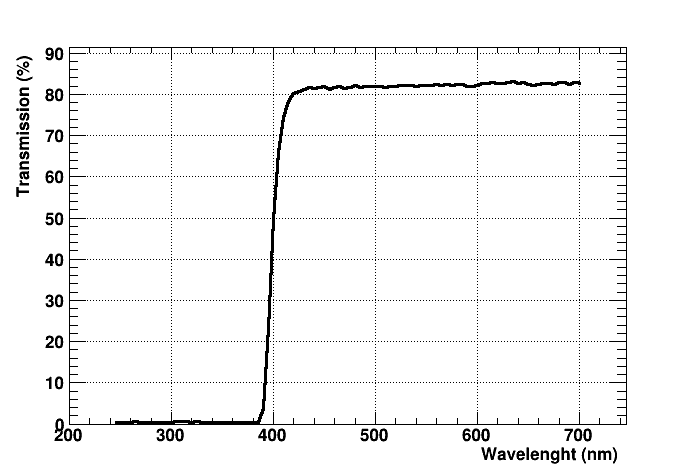
\includegraphics[width=7cm]{../Pictures/Chapter_5/lso_trans.png}
\end{center}
\caption[Transmission curve for LuAG and LSO]{Transmission curve for a LuAG:Ce (left) and a LSO:Ce (right) sample.}
\label{fig:luag_lso_trans}
\end{figure}

\begin{figure}[htbp]
\begin{center}
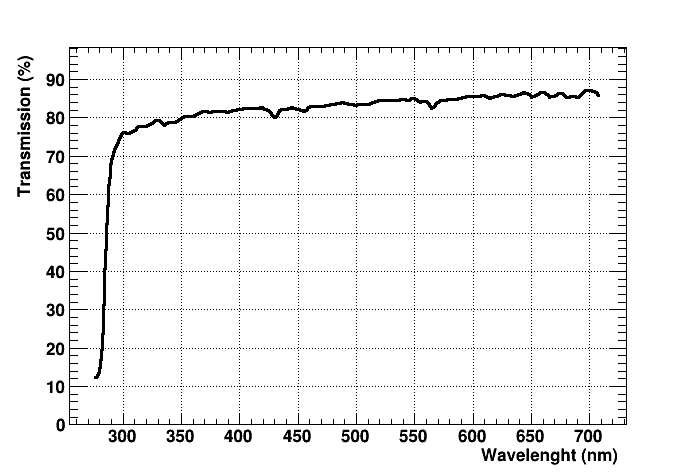
\includegraphics[width=7cm]{../Pictures/Chapter_5/cef3_trans.png}
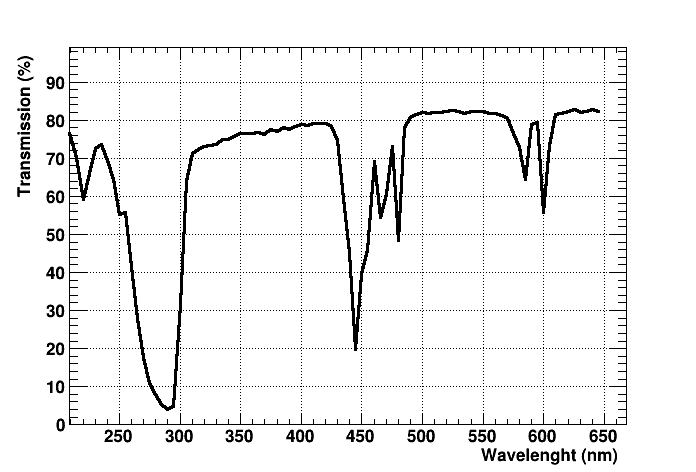
\includegraphics[width=7cm]{../Pictures/Chapter_5/luag_pr_trans.png}
\end{center}
\caption[Transmission curve for LuAG CeF$_{3}$]{Transmission curve for a CeF$_{3}$ (left) and a LuAG:Pr (right) sample.}
\label{fig:cef_pr_trans}
\end{figure}

\subsection{Light yield}
The definition of light yield has been already given in chapter 2, as well as considerations on the difference between absolute light yield and light output in a specific configuration. The setup for light yield measurement is shown in figure \ref{fig:set_LY}. 
Teflon tape was used as a reflector, for the case of light yield measurement as well as the $\gamma$ rise time measurement. 
\begin{figure}[htbp]
\begin{center}
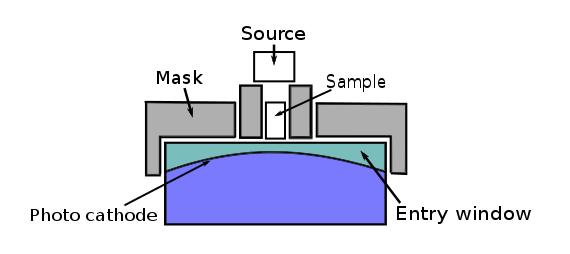
\includegraphics[width=8cm]{../Pictures/Chapter_5/LY_3.png}
\end{center}
\caption[Light Yield setup]{Set up for the measurement of light yield.}
\label{fig:set_LY}
\end{figure}
The presence of wrapping allows to couple out more photons, and in a few cases this is necessary to infer the light output (given the low intrinsic light yield), at the cost of a minor repeatability of the measurement. The experimental error was checked with repetition of the measurement, and estimated around 5$\%$.
The light output has been measured with a $^{137}$Cs source ($E_{\gamma}$ = 662 keV) placed a few mm above the crystal. The system crystal-PMT was placed inside a black box, with controlled temperature ($20^{\circ}C$) to avoid drift in the system response.
Further shielding against background light was ensured by an aluminium cap covering the entry window of a Hamamatsu R2059 PMT.
After the collection of the photo electrons at the anode of the PMT, the signal is attenuated, shaped and stored by the DAQ, with a digitizer \textit{CAEN DT$5720$}.

To measure the light output of sample crystals the number of photo electrons $N_{pe}$ collected can be used.
In particular by computing the area of the scintillation pulse we can obtain the number of photo-electrons collected by comparison with the value of the single electron response (SER).
The SER is measured exploiting the dark current of the PMT, caused by thermal emission of electrons from the photo cathode.
After multiplication in the dynode system, the charge integrated is the response of the PMT to a single photo electron.
The probability to emit two electrons is very low.
The number of photo electrons can be calculated by comparing the position of the photo electric peak with the spectrum that characterizes a single photon emission. The number of photo electrons produced per impinging MeV can be determined as
\begin{equation}
N_{pe}/MeV=\frac{position\ photo\ peak}{position\ single\ photo\ electron\ peak} \cdot \frac{A_{1}}{A_{2}} \cdot \frac{1}{E_{\gamma}}
\end{equation}
where $E_{\gamma}$ is the energy of the incident $\gamma$ particle and linearity of the detector response is assumed. A pedestal may be subtracted from the position of the peaks. $A_{1}$ and $A_{2}$ are the values of the attenuation of the signal in the case of the photo peak and the single electron peak, i.e.
\begin{equation}
A_{i}=e^{\frac{B_{i}}{20}}
\end{equation}
and $B_{i}$ is the attenuation in dB.
In order to extract the position of the photo peak and the resolution on the peak  from the charge spectra, the sum of a Gaussian and a Fermi distribution is used for the fit:
\begin{equation}
y(x)=\frac{P}{e^{\frac{x-C}{R}}+1}+Ae^{-\frac{(x-\mu)^{2}}{2\sigma ^{2}}}
\end{equation}
where P, C and 1/R correspond to height, position and slope of the Compton edge, A is the height of the photo peak with position $\mu$ and FWHM width 2.35 $\sigma$.
For the single photo electron spectrum a simple Gaussian fit determines the charge for the single photon with sufficient accuracy, at 1.6 pC.
An example of the light yield spectrum the single photo electron spectrum are shown in figure \ref{fig:spectrum}.

At this point the number of photons extracted per MeV can be determined if the quantum efficiency of the photo detector is known:
\begin{equation}
N_{ph}/MeV=\frac{N_{pe}}{QE}
\end{equation}
In order to determine the average quantum efficiency given a certain sample, the emission curve of the sample itself was used, and weighted by the quantum efficiency curve of the PMT (shown in figure \ref{fig:QE}).
Finally the integration time was optimised on the time profile of the crystal measured, so that for LSO was set to 400 ns and for LuAG to 4 $\mu$s.

To correct for long-term variations of the PMT gain and quantum efficiency, the light output of a reference crystal is used. In order to guarantee repeatability the crystal is encapsulated into Teflon to protect it and fix the position with respect to the photocathode and the source. The sample is a is $2\times 2\times 10$ $mm^{3}$ LuAP crystal.
The samples measured and relative size are shown in table \ref{table:LYtable} along with the result obtained. Some crystals present such a low light output that it was not possible to infer the photopeak position in a naked configuration. The only available data point is with Teflon wrapping.

\begin{figure}
\begin{center}
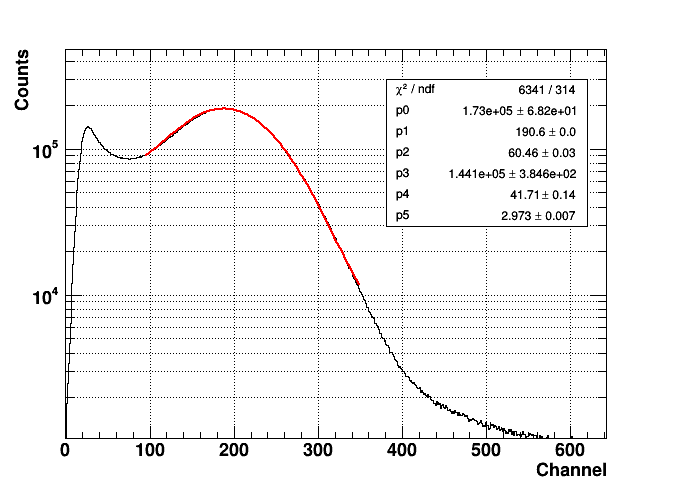
\includegraphics[width=9cm]{../Pictures/Chapter_5/single.png}
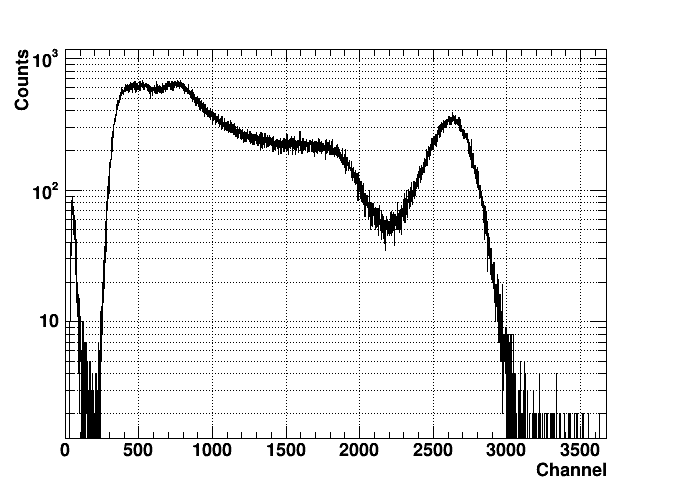
\includegraphics[width=9cm]{../Pictures/Chapter_5/spectrum_LY.png}
\end{center}
\caption[Single electron and LSO $^{137}$ Cs spectrum]{Spectrum fit with Gaussian for single photo electron peak (top) and $^{137}$ Cs spectrum for LSO:Ce crystal (bottom)}
\label{fig:spectrum}
\end{figure}

\begin{figure}
\begin{center}
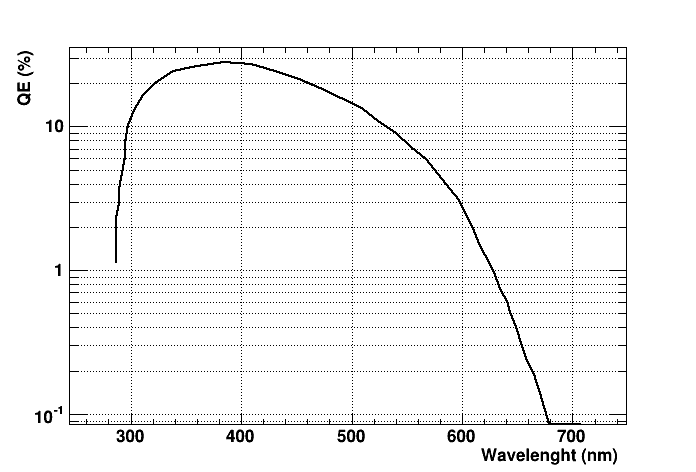
\includegraphics[width=9cm]{../Pictures/Chapter_5/qe.png}
\end{center}
\caption[QE of R2059 PMT]{Quantum efficiency curve for the Hamamatsu R2059 PMT}
\label{fig:QE}
\end{figure}

% come lo determino? da vedere!
\begin{table}[h]
\begin{center}
\begin{tabular}{|l|l|l|l|l|l|}
\hline
Crystal  & L0 (Teflon) & Res (Teflon) & LO (naked) &  Res(naked) & QE\\
\hline
LSO:Ce,Ca& 8536&15 & 3456&16 &0.22\\
\hline
LYSO:Ce (Sipat)&11002 &15 &4814 &16&0.22\\
\hline
LYSO:Ce (Proteus)& 13879& 12.9 & 4692& 17.3&0.22\\
\hline
LSO:Ce (CTI)&15583 &11.9 &5200 &14&0.22\\
\hline
LGSO:Ce & 10255&13.7 &3934 &14.1&0.22\\
\hline
CeF$_{3}$&2300&26 & & &0.22\\
\hline
LuAG:Ce (0.13$\%$)&6800 &16 & & &0.1\\
\hline
BGO&6500 &11 & & &0.16\\
\hline
\end{tabular}
\end{center}
\captio[Light yield values for the samples measured]{Light yield measured for the samples naked and Teflon wrapped}
\label{table:LYtable}
\end{table}

